\documentclass{article}
\usepackage{ijcai17}
\usepackage{times}

%\usepackage{pdfinfo}

% \usepackage{latexsym} 
\pdfinfo{
/Title (Nash Equilibria in Games with Lexicographic Goals)
/Author (TBA)}

\title{Nash Equilibria in Games with Lexicographic Goals}

%\title{Rational Cost Games}
%\title{Nash Equilibria in Games with Combined Qualitative and Quantitative Goals}


\author{XXX}



% % \usepackage{times,mathtools}
% % \usepackage{latexsym,upgreek,wasysym,graphicx,textcomp}
 \usepackage{xspace,color,upgreek}
% % \usepackage[inline]{enumitem}
%% PACKAGES %%
%\usepackage{latexsym}
\usepackage{amsmath}
\usepackage{amssymb}
%\usepackage{amsthm}


\usepackage{xspace,color,hyperref,upgreek} 
\usepackage{graphicx}
\usepackage{tikz,pgf}
\usetikzlibrary{arrows,shapes,automata,positioning,matrix,calc,petri}

%% ENVIRONMENTS %%
%\theoremstyle{plain}
%\newtheorem{theorem}{Theorem}
%\newtheorem{lemma}{Lemma}
%\newtheorem{fact}{Fact}
%\newtheorem{example}{Example}
%\newtheorem{definition}{Definition}
%\newtheorem{corollary}{Corollary}
%\newtheorem{proposition}{Proposition}
%\newtheorem*{proof*}{Proof}

%% COMMENTS %%

%\newcommand\note[1]{{\color{red}{#1}}}

\newcommand\sr[1]{{\color{red}{(sr:#1)}}}
% \renewcommand{\sr}[1]{}
\newcommand\ba[1]{{\color{purple}{(ba:#1)}}}
\newcommand\fz[1]{{\color{blue}{(fz:#1)}}}

\newcommand{\todo}[1]{{{\color{blue} #1}}}
%\renewcommand{\todo}[1]{}

%% LATEX SHORTCUTS %%

\def\it{\begin{itemize} }
\def\-{\item }
\def\ti{\end{itemize} }
\def\en{\begin{enumerate} }
\def\ne{\end{enumerate} }

%% COMPLEXITY CLASSES %%


\def\exptime{\textsc{exptime}\xspace}
\def\exptimeC{\exptime-complete}

\def\expspace{\textsc{expspace}\xspace}

\def\pspace{\textsc{pspace}\xspace}
\def\pspaceC{\pspace-complete}

\def\logspace{\textsc{logspace}\xspace}
\def\nlogspace{\textsc{nlogspace}\xspace}

\def\ptime{\textsc{ptime}}
\def\np{\textsc{np}}



%% LOGIC %%
\def\fol{\mathsf{FOL}}
\def\msol{\ensuremath{\mathsf{MSOL}}\xspace}
\def\fotc{\mathsf{FOL+TC}}

%% TEMPORAL LOGIC %%
\newcommand{\sqsq}[1]{\ensuremath{[\negthinspace[#1]\negthinspace]}}

\DeclareMathOperator{\ctlE}{{\mathsf{E}}}
\DeclareMathOperator{\ctlA}{\mathsf{A}}

\newcommand{\atlE}[1]{\ensuremath{\langle\!\langle{\text{#1}}\rangle\!\rangle}}
\newcommand{\atlA}[1]{\ensuremath{[\:\!\![\text{#1}]\:\!\!]}}

\DeclareMathOperator{\nextX}{\mathsf{X}}
\DeclareMathOperator{\yesterday}{\mathsf{Y}}
\DeclareMathOperator{\until}{\mathbin{\mathsf{U}}}
\DeclareMathOperator{\weakuntil}{\mathbin{\mathsf{W}}}
\DeclareMathOperator{\since}{\mathbin{\mathsf{S}}}
\DeclareMathOperator{\releases}{\mathbin{\mathsf{R}}}
\DeclareMathOperator{\always}{\mathsf{G}}
\DeclareMathOperator{\hitherto}{\mathsf{H}}
\DeclareMathOperator{\eventually}{\ensuremath{\mathsf{F}}\xspace}
\DeclareMathOperator{\previously}{\mathsf{P}}
\newcommand{\true}{\mathsf{true}}
\newcommand{\false}{\mathsf{false}}


\newcommand{\LTL}{\ensuremath{\mathsf{LTL}}\xspace}
\newcommand{\PLTL}{\textsf{PROMPT-}\LTL}

\newcommand{\CTL}{\ensuremath{\mathsf{CTL}}\xspace}
\newcommand{\CTLS}{\ensuremath{\mathsf{CTL}^*}\xspace}
\newcommand{\PCTLS}{\textsf{PROMPT-}\CTLS}
\newcommand{\PCTL}{\textsf{PROMPT-}\CTL}
\newcommand{\CLTL}{\ensuremath{\textsf{C-}\LTL}\xspace}
\newcommand{\PCLTL}{\ensuremath{\textsf{PROMPT-C}\LTL}\xspace}

\newcommand{\ATL}{\ensuremath{\mathsf{ATL}}\xspace}
\newcommand{\ATLS}{\ensuremath{\mathsf{ATL}^*}\xspace}
\newcommand{\PATLS}{\textsf{PROMPT-}\ATLS}
\newcommand{\PATL}{\textsf{PROMPT-}\ATL}


\def\alt{\, | \,}


\DeclareMathOperator{\Fp}{\eventually_\mathsf{P}}

\newcommand{\AP}{\mathrm{A\!P}}

%% MATH OPERATIONS %%
\newcommand{\tpl}[1]{\langle {#1} \rangle }
\newcommand{\tup}[1]{\overline{#1}}


%% STRUCTURES %%
\newcommand{\LTS}{\mathsf{S}}
\newcommand{\Paths}{\mathsf{pth}}
\newcommand{\nat}{\mathbb{N}}
\def\int{\mathbb{Z}}
\newcommand{\natzero}{\mathbb{N}_0}

\newcommand{\trans}[3]{#1 \stackrel{{#3}}{\rightarrow} #2}


%% HEADINGS ETC %%
\newcommand{\head}[1]{\noindent{\bf #1}}

%% COUNTER MACHINES %%
\newcommand{\cm}{\ensuremath{M}}
\newcommand{\CMinc}{\mathsf{inc}}
\newcommand{\CMdec}{\mathsf{dec}}
\newcommand{\CMzero}{\mathsf{ifzero}}
\newcommand{\CMnonzero}{\mathsf{nzero}}
\newcommand{\CMcommit}{\mathsf{end}}


%% CLTL %%
\def\var{{\sf var}}
\def\ovar{{\sf ovar}}
\def\avar{{\sf avar}}
\def\svar{{\sf svar}}
\def\bvar{{\sf bvar}}

\def\MOD{\equiv}

%% PVP %%
\def\PVP{\mathsf{PVP}}





\def\hist{{\sf Hst}} %history
\def\plays{{\sf Ply}} %plays



\def\DCLPC{{\sf{DCL-PC}}}
\def\ATL{{\sf{ATL}}}
\def\ATLS{{\sf{ATLS}\xspace}}
\def\CTLS{{\sf{CTLS}\xspace}}
\def\CLPC{{\sf{CL-PC}}}
\def\LCGS{{\sf LCGS}\xspace}
\def\CGS{{\sf CGS}\xspace}
\def\cgs{\CGS}
\def\CCGS{{\sf CCGS}\xspace}
\def\CCGA{{\sf CCGA}\xspace}

\def\Pth{{\sf Pth}} %set of plays
\def\playf{{\sf play}}
\def\Reach{{\sf Reach}}
\newcommand{\Hst}{{\sf Hst}}
\newcommand{\St}{St}
\newcommand{\Str}{{\sf Str}}
\newcommand{\exec}{{\sf Exec}}

\def\mp{{\sf mp}}
\def\max{{\sf max}}
\def\parity{{\sf parity}}

\newcommand\card[1]{|{#1}|}

\newcommand{\C}{{\mathfrak{C}}}

%LOGICS 
\newcommand{\LATL}{{\sffamily LATL}\xspace}
\newcommand{\LATLS}{{\sffamily LATLS}\xspace}


\def\lex{\prec_{lex}}
\def\lexeq{\preceq_{lex}}
\def\LEX{{\sf Lex}}

\def\NE{{\sf NE}}


\newcommand{\longtrans}[3]{#1 \stackrel{\mathsf{#3}}{\leadsto} #2}
\newcommand{\longtranszero}[3]{#1 \stackrel{\mathsf{#3}}{\leadsto_0} #2}
%\newcommand{\todo}[1]{{{\color{blue} (#1)}}}

\newcommand{\coop}[2][]{\langle\!\langle{#2}\rangle\!\rangle_{_{\!\mathit{#1}}}}

\newcommand{\noavoid}[1]{[\![{#1}]\!]}




\begin{document}




\section*{Decisions}

We agreed i) to have weights on actions and a note/remark about the extension to weights on states or edges; ii) to focus on NE for arbitrary strategies and, if we can prove something useful/interesting, $\epsilon$-NE for finite-memory strategies; iii) we probably have enough material with mean-payoff and can consider max for a journal version; iv) it is probably enough to focus on the following decision problems: NE-emptiness, E-Nash, NE-membership.


\section*{Todos}

\begin{enumerate}
 \item Settle on structure of paper

 \item Fill in the details of the proof sketches already in the draft. Note that bisimilar CGSs may not preserve existence of NE if histories are sequences of states. However, if histories alternate states and actions, then indeed they do. So, we must carefully check the papers we cite/use.

 \item Decide if we want LTL or Lex formulas $\Phi$ for E-Nash. Question: how does one motivate E-Nash with LEX objectives for the government? Potential answer: social welfare. Technically, add an extra component to each tuple of actions in the CGS that belongs to the government.
  
 \item Instead of reducing E-Nash to NE-emptiness it seems that one can simply adapt the proof that NE-emptiness is decidable for Lex Games to proving that E-Nash is decidable for Lex Games. Indeed, instead of looking for a secure path in G', look for a secure path in G' that satisfies the given formula $\Phi$. Also, Giuseppe 
checked that E-Nash reduces to NE-emptiness using the usual matching-pennies gadget. We should decide whether to present NE-emptiness or E-nash ``first''.


 \item Discuss ``motivating examples''/``applications''.  Example scenario: i) one wholesaler and a bunch of retailers, each trying to maximise profit (this needs to be formalised); ii) taxation schemes. Perhaps look at motivating examples from papers on mean-payoff games for ideas.
 
 \item If we need extra: If we need more dec probs, we might look at strong NE; other restrictions on strategy memory, myopic.
 
 \item Absorb definition and techniques for $\epsilon$-Nash equilibria.
\end{enumerate}

\clearpage

\maketitle

\section{Introduction}

\section{Background}  \label{sec:prelim}
We will use basic notions from mathematical logic including monadic second-order logic~\cite{EbFl95}, automata theory~\cite{HMU03}, 
and linear-temporal logic~\cite{CGP1999}. We will introduce them below, as needed.
%, and the theorem of McNaughton and Papert connecting star-free languages and first-order logic, see~\cite{Thomas96})
%
Write $B^\omega$ for the set of infinite sequences over alphabet $B$, and write $B^*$ for the set of finite sequences. The empty sequence is denoted $\epsilon$.
Sequences are indexed starting at $0$, thus we write $\alpha = \alpha_0 \alpha_1  \cdots$. 
Write $[n]$ for the set $\{1,2,\cdots,n\}$.

\todo{In the rest of this paper we use the term ``robot'' instead of ``mobile agent''.}

% The reader may refer to this section as needed.
\subsection{Graphs, \LTL and \msol} \label{subsec:graphs-MSOL}

\head{Graphs.} Graphs will serve as the environment in which robots move.
Let $\Sigma$ be a finite set of {\em edge labels}.
A {\em $\Sigma$-graph}, or {\em graph}, $G$, is a tuple $(V,\lambda)$ where $V$ is a finite set of {\em vertices} and $\lambda:V^2 \to \Sigma$ is a partial function called the {\em edge labeling function}. The domain of $\lambda$ is denoted $E \subseteq V \times V$, and is called the
{\em edge relation}. We write $\trans{v}{w}{\sigma}$ to mean $\lambda(v,w) = \sigma$.
A graph is \emph{deterministic} if for every $v \in V, \sigma \in \Sigma$ there exists at most one $v'$ such that $\lambda(v,v') = \sigma$. Here are some examples of classes of deterministic graphs.

% \sr{Q: do we want to consider nondeterministic graphs? what about vertices from which there may not be an edge labeled $\sigma$?}

%The {\em out-degree} of a vertex $v$, written $\deg(v)$, is the cardinality of the set $\{(v,w) \in E : w \in V\}$ of {\em outgoing edges} of $v$.
%
%Sometimes the edge labels give a sense of direction:
%
%\begin{example} An {\em $L$-labeled grid} is a graph with $V = [n] \times [m]$, $\Sigma =  L \times \{N,S,E,W\}$, and labels $\lambda((x,y),(x+1,y)) \in L \times \{E\}$, etc., where $L$ is a finite set and $n,m \in \nat$. An {\em $L$-labeled line} is an $L$-labeled grid with $V = [n] \times [1]$. If $|L| = 1$ then we call the grid (or line) {\em unlabeled}.
%\end{example}
%


% \label{ex:tree}
\head{Trees.} A {\em $\Delta$-ary tree} (for $\Delta \in \nat$) is a $\Sigma$-graph $(V,\lambda)$ where $(V,E)$ is a tree, $\Sigma = [\Delta] \cup \{up\}$, and $\lambda$ labels the edge leading to the node in direction $i$ (if it exists) by $i$, and the edge leading to the parent of a node (other than the root) is labelled by $up$. We may rename the labels for convenience, e.g., for binary trees ($\Delta = 2$) we let $\Sigma = \{lc,rc,up\}$ where $lc$ replaces $1$ and $rc$ replaces $2$. For instance, see Figure~\ref{fig:tree}.

\head{Lines.} The \emph{$n$th line} is the $\Sigma$-graph $L_n = (V_n,\lambda_n)$, where $\Sigma = \{l,r\}$, $V_n = [n]$, and $\lambda_n(i,i+1) = r$ and $\lambda_n(i+1,i) = l$. Thus, the domain of $\lambda_n$ is  $E_n = \cup_{i,j \in [n]} \{(i,j) : |i-j| = 1\}$. \label{def:line}

\head{Grids.} The \emph{$n$th grid} is the $\Sigma$-graph $G_n = (V_n,\lambda_n)$, where $\Sigma = \{u,d,l,r\}$, $V_n = [n] \times [n]$,  and the labels are as expected with $u$ standing for ``up'', $d$ for ``down'', $l$ for ``left'' and $r$ for ``right''. E.g., $\trans{(i,j)}{(i+1,j)}{r}$ and $\trans{(i,j)}{(i,j+1)}{u}$.
% Thus the edge relation $E_n$ consists of all pairs $((i,j),(i',j'))$ such that $|i-i'| = 1$ xor $|j = j'| = 1$.

%A $\Delta$-ary tree with $\Delta = 1$ is called a {\em line}. A $\Delta$-ary tree in which every vertex has degree at most $2$ is called a {\em labelled line}.


% The degree of a graph $G$ is the maximum degree of all its vertices.


% To simplify the presentation we do not distinguish between the syntactic symbols used in formulas (such as the binary relation symbol $E$) and the semantic symbols used in structures; thus, e.g., we write the formula $E(x,y)$ where $E$ is a binary relation symbol, as well as the expression $(u,v) \in E$ where $E$ is the edge relation of a graph.


\head{Linear Temporal Logic.} \label{dfn:LTL}
This is a canonical modal logic for the specification of reactive systems. Here we will use it as a foundation for specifying robot tasks.

For a set of \emph{atoms} $\AP$, write $\LTL(\AP)$ (or simply \LTL) for the logic with the following syntax and semantics:
$\varphi ::= p \mid \varphi \wedge \varphi \mid \neg \varphi \mid \nextX \varphi \mid \varphi \until \varphi$, where $p$ varies over $\AP$.
We use standard abbreviations, e.g., $\false := p \wedge \neg p, \true := \neg \false, \eventually \varphi := \true \until \varphi$,
	$\always \varphi := \neg \eventually \neg \varphi$, etc.
% 	 $\varphi \weakuntil \varphi' := (\varphi \until \varphi') \vee \always \varphi$,
	The \emph{safety} formulas are those of the form $\always b$ where $b$ is a Boolean combination of atoms.
	
	
	Formulas are interpreted over infinite strings $\alpha = \alpha_0 \alpha_1 \alpha_2 \cdots \in (2^\AP)^\omega$. Define the satisfaction relation
	$\models_\LTL$ as follows:
	\it
	\- $(\alpha,n) \models_\LTL p$ iff $p \in \alpha_n$;
	\- $(\alpha,n) \models_\LTL \varphi_1 \wedge \varphi_2$ iff $(\alpha,n) \models_\LTL \varphi_i$ for $i = 1,2$;
	\-	$(\alpha,n) \models_\LTL \neg \varphi$ iff it is not the case that $(\alpha,n) \models_\LTL \varphi$;
	\-  $(\alpha,n) \models_\LTL \nextX \varphi$ iff $(\alpha,n+1) \models_\LTL \varphi$;
	\- $(\alpha,n) \models_\LTL \varphi_1 \until \varphi_2$ iff there exists $i \geq n$ such that $(\alpha,i) \models_\LTL \varphi_2$ and for all $i \leq j < n$, $(\alpha,j) \models_\LTL \varphi_1$.
	\ti
	Write $\alpha \models_\LTL \varphi$ if $(\alpha,0) \models_\LTL \varphi$ and say that $\alpha$ \emph{satisfies} $\varphi$.



  \head{Monadic Second-order Logic.} \label{dfn:msol} This is an extension of first-order logic by set variables. It will be used to define powerful testing abilities of robots, as well as a technical tool in the decidability proofs.

Formulas are interpreted in $\Sigma$-graphs $G$. Define the set of monadic second-order formulas $\msol(\Sigma)$ as follows. Formulas of $\msol(\Sigma)$ are built using {\em first-order variables} $x,y,\cdots$ that vary over vertices, and {\em set variables} $X,Y, \cdots$ that vary over sets of vertices. The {\em atomic formulas} (when interpreted over $\Sigma$-graphs) are:
\it
\- $x = y$ (denoting that vertex $x$ is the same as vertex $y$),
\- $x \in X$ (denoting that vertex $x$ is in the set of vertices $X$),
% \- $init(x)$ (denoting that $x$ is the initial vertex $v_0$), and
\- $\lambda(x,y) = \sigma$ (denoting that there is an edge from $x$ to $y$ labeled $\sigma \in \Sigma$).
% \- $\true$ (the formula that is always true).
\ti
The formulas of $\msol(\Sigma)$ are built from the atomic  formulas using the Boolean connectives (i.e., $\neg,\vee, \wedge, \limp$) and variable quantification (i.e., $\forall,\exists$ over both types of variables). The fragment of $\msol(\Sigma)$ which does not mention set variables is called {\em first-order logic}, denoted $\fol(\Sigma)$.
Write $\msol_k(\Sigma)$ for formulas with at most $k$ many free first-order variables and no free set-variables. We abbreviate $z_1, \cdots, z_k$ by $\tup{z}$. We write $\phi(x_1, \cdots, x_k)$ to mean that the free variables from the formula $\phi$ are amongst the set $\{x_1, \cdots, x_k\}$. Note that the formula $\phi(x_1,\cdots,x_k)$ does not need to use all the variables from the set $\{x_1,\cdots,x_k\}$. When $\Sigma$ is clear from the context, it may be dropped.

The semantics of \msol is defined in a similar way as for first-order logic. Instead of giving the formal definitions (see~\cite{EbFl95}) it is enough to introduce some useful notation. Given a graph $G$, a \emph{valuation $\nu$} is a function that maps each first-order variable to a vertex in $G$ and each monadic second-order variable to a set of vertices of $G$. Thus, we write $(G,\nu) \models \phi(x_1,\cdots,x_k,X_1, \cdots, X_l)$ to mean that $\phi$ holds in $G$ with variable $x_i$ (resp. $X_i$) simultaneously substituted by vertex $\nu(x_i)$ (resp. $\nu(X_i)$).
A {\em sentence} is a formula with no free variables. In this case we write $G \models \phi$ to mean that $\phi$ holds in $G$. A sentence $\phi$ is \emph{satisfiable} if there exists a graph $G$ such that $G \models \phi$.



%  A sentence $\phi$ is \emph{valid} if for all graphs
%  $G$, $G \models \phi$.
% \sr{remove dfns of sat and valid if they are not needed}


%\footnote{In the section on \RLTL\ we will introduce the satisfaction relation $\models_{\tup{R},\Omega}$.}

Here are some examples of formulas and their meanings:
\example{\label{ex:formulas}
\begin{itemize}

% \item  We abbreviate $\bigwedge_i x_i = y_i$ by $\tup{x} = \tup{y}$, and $\bigwedge_i x_i \in X_i$ by $\tup{x} \in \tup{X}$.

\item The formula $\forall x (x \in X \limp x \in Y)$ means that $X \subseteq Y$. Similarly, there are formulas for the set operations $\cup, \cap,=$, and relative complement $X \setminus Y$.

 \item The formula $E(x,y) := \bigvee_{\sigma \in \Sigma} \lambda(x,y) = \sigma$ says that there is an edge from $x$ to $y$.

 \item On lines (so $\Sigma = \{l,r\}$) the formula $\neg \exists y. \lambda(x,y) = r$ states that $x$ is on the right end-point of the line.

 \item On binary-trees (so $\Sigma = \{lc,rc,up\}$) the formula $\neg \exists y. \lambda(y,x) = up$ states that $x$ is a leaf, $\neg \exists y. \lambda(x,y) = up$ states that $x$ is the root, and $\exists y. \lambda(y,x) = lc$ states that $x$ is a left-child.

%\item The formula $\exists x \exists y (x\neq y \wedge  edg(z,x) \wedge edg(z,y))$ means that $\deg(z) \geq 2$.
 \item The formula $E^*(x,y) := \forall Z [(closed_{E}(Z) \wedge x \in Z) \limp y \in Z]$ defines the transitive closure of $E$, where $closed_{E}(Z)$ is $\forall a \forall b[(a \in Z \wedge E(a,b)) \limp b \in Z]$.


%  $\phi^*(x,y)$ holds in a graph $G$ if and only if there exists a finite sequence of vertices $v_1 v_2 \cdots v_m \in V^*$  (here $m \geq 1$) such that $x = v_1, y = v_m$ and $\phi(v_i,v_{i+1})$ holds in $G$ for all $i < m$ (for example, if $\phi(x,y) = edg(x,y)$ then $G \models \phi^*(x,y)$  if and only if $G$ has a path from $x$ to $y$). This shows that that if a binary relation is $\msol$-definable, then so is its transitive-closure.
% %%Write $[[\phi]]_G := \{\tup{v} \in V^k : G \models \tup{v}\}$.
%%We say that a graph $G$ {\em satisfies} a sentence $\phi$, and write $G \models \phi$, if $\phi$ is true in the graph $G$.
\end{itemize}
}
% of $\msol$-definable formulas \label{ex:TC} \begin{itemize}
%\item
%
%
%
%%Similarly, $\phi^+(x,y) := \exists z (\phi(x,z) \wedge \phi^{*}(z,y))$ is as before, but replace $m \geq 1$ by $m > 1$.
%\item Similarly, define $\phi^\omega(x,y) := \phi^*(x,y) \wedge \exists z (\phi(y,z) \wedge \phi^{*}(z,y))$. Note $\phi^\omega(x,y)$ holds in a graph $G$ if and only if there is an infinite sequence of vertices $v_1 v_2 \cdots \in V^\omega$ with $x= v_1$, $v_i = y$ for infinitely many $i \in \nat$, and $\phi(v_i,v_{i+1})$ holds in $G$ for all $i \in \nat$. This uses the fact that $V$ is finite.
%
%\item Note that if $\phi(x,y,\tup{z})$ is an $\msol(\Sigma)$ formula we can define an $\msol(\Sigma)$ formula $\phi^*(x,y,\tup{z})$ that expresses  that there exists a finite sequence of vertices $v_1 v_2 \cdots v_m \in V^*$  (here $m \geq 1$) such that $x = v_1, y = v_m$ and $\phi(v_i,v_{i+1},\tup{z})$ holds in $G$ for all $i < m$. In other words, we can treat $\tup{z}$ as parameters. We can similarly add parameters to $\phi^\omega$.
%\end{itemize}

%no space
%\item[MF5.] \label{ex:ktc}


%The set of formulas in $\fotc(\Sigma)$ is defined to be the set of formulas $\fol(\Sigma)$  closed under the transitive-closure operator (for $k=1$). We have seen that every formula in $\fotc(\Sigma)$ is expressible as a formula in $\msol(\Sigma)$, which justifies writing $\fotc(\Sigma) \subset \msol(\Sigma)$, a slight abuse of notation. \sr{is FOTC used?}






%\subsection{Automata and Regular Expressions.}
%\sr{define automata? universality problem?}
%
% Ordinary {\em regular-expressions} over a finite alphabet $B$ are built from the
% sets $\emptyset$, $\{\epsilon\}$, and $\{b\}$ ($b \in B$), and the operations
% union $+$, concatenation $\cdot$, and Kleene-star $\phantom{}^*$.
% Kleene's Theorem states that the languages definable by regular expressions over
% alphabet $B$ are exactly those recognised by finite automata over alphabet $B$.


%
% An {\em $\omega$-regular expression} over alphabet $B$ is inductively defined to
% be of the form: $exp^\omega$, $exp \cdot r$, or $r + r'$, where $exp$ is an
% ordinary regular-expression over $B$, and $r,r'$ are $\omega$-regular
% expressions over $B$. An {$\omega$-regular language} is one defined by an
% $\omega$-regular expression. A variation of Kleene's Theorem says that the
% languages definable by $\omega$-regular expressions over alphabet $B$ are
% exactly the languages recognised by B\"uchi automata over alphabet $B$ (which
% are like finite automata except they take infinite words as input, and a run is successful if
% some accepting state occurs infinitely often).


%A regular language over alphabet $B$ is {\em star-free} if it is the language of a regular-expression over $B$ that does not use the Kleene-star, but may use the complementation operator (written $\neg{r}$).
%A {\em star-free $\omega$-regular language} is the language of an $\omega$-regular expression that may mention the complement operator, but may not mention the $\omega$-power $exp^\omega$ nor the Kleene-star $exp^*$ operators.

\iffalse
We will use the McNaughton-Papert Theorem (and its generalisation to infinite-words) (see \cite{Thomas96,DiGa08}): it states that a regular language of ($\omega$)-words is star-free if and only if it is definable in first-order logic. For instance, the language $0^*1^*$ over alphabet $\{0,1\}$ is definable by the formula $\exists z. \forall x. [x \leq z \limp P_0(x)] \wedge [x \not \leq z \limp P_1(x)]$, and by the star-free regular expression $\neg( \neg{\emptyset} \cdot 1 \cdot 0 \cdot  \neg{\emptyset})$. Formally, a word $w \in B^*$ is coded as a structure with domain $[|w|]$, unary predicates $P_b := \{i \leq |w| : w_i = b\}$ (for $b \in B$), and the usual linear order $\leq$ on $[|w|]$; and thus the first-order definition may make use of these unary predicates and the linear order.
\fi

%\footnote{Although this is the standard encoding, if one prefers uniformity with the earlier definition graph, one may instead code the word $w$ as an edge-labeled graph with $|w|+1$ vertices, and an additional edge label for $\leq$.}

%\sr{use 'FO language' and 'FO models'?}
%Graphs of degree at most $\Delta \in \nat$ will be called $\Delta$-graphs.


\section{The Model of Multi-Robot Systems and Robot Task Logic} \label{sec:model}


In this section we provide a framework for modeling multi-robot systems parameterised by their environment. Here is a brief outline.
%We generalise the definition of robot systems from \cite{Rubin15AAMAS} to allow asynchronous behaviour.
An environment is modeled as a $\Sigma$-graphs $G$, and robots are modeled as finite-state automata over an alphabet of guarded commands.
A guarded command tells the robot to move along an edge with a given label or stay where it is, subject to a test being true.
Robots can test their own current positions, as well as the published positions and local states of other robots. That is, robots can publish their current
position and local state (by entering special `publishing' states) --- this can be thought of as shared memory, or a bulletin-board, where each robot overwrites
its current state and position. Robots move asynchronously, i.e., at least one robot (chosen nondeterministically) moves at a time.
We also provide a definition of a logic, based on Linear Temporal Logic (\LTL), in which one can express various tasks such as gathering, exploring, and reconfiguring.  The logic is called Robot Linear Temporal Logic (\RLTL): it is like \LTL except that its atoms are tests. We assign one \RLTL formula to each robot that specifies its goal, and we require that each of the robots achieve its goal. Thus, co-operative global specifications are given by specifying the individual requirement for each robot.
%e.g., to specify that all robots gather we assign to each robot the individual task of reaching a position containing all the other robots.
% All tests (whether for robots or specfication formula) are based on \msol.
%As discussed in Section~\ref{sec:DC}, our model is general enough to be able to express a popular model of robot systems found in the distributed computing literature~\cite{FIPPP04,Diks200438,Cohen05graphexploration,KKR06,GR08,Das13}.

\subsection{The Model of Multi-Robot Systems}

In the rest of this section, $\Sigma$ denotes a finite set of edge-labels, and $k \in \nat$ denotes the number of robots.

\head{Commands and Tests.}
%
A {\em command} is a symbol from $\upmu(\Sigma) := \{move(\sigma) : \sigma \in \Sigma\} \cup
\{stay\}$.  The command $move(\sigma)$ tells the robot to move
from its current vertex along an edge labeled $\sigma$, and the command
$stay$ tells the robot to stay at its current vertex.

% \sr{should we instead use $pub\_{pos_i}$, $cur\_pos$, $pub\_{st_i}$, $cur\_st$? no.}

% \sr{i changed $cur$ to $pos_{cur}$.}

 A {\em position-test} is a formula $\tau$ from $\msol_{k+1}(\Sigma)$ whose free variables come from the set 
 $\{\VARbcpos_1, \cdots, \VARbcpos_k,\VARpos_{cur}\}$. Informally, a position test
  \[
\tau(\VARbcpos_1,\cdots,\VARbcpos_k,\VARpos_{cur})  
 \]
allows the robot to test that $\tau$ holds in $G$
 where $\VARbcpos_{cur}$ is the current position of the robot doing the testing, and each $\VARbcpos_i$ is the last published position of the $i$th robot.
 Thus, the test $\VARbcpos_i = \VARbcpos_{cur}$ states that the current position (of the robot doing the testing) is equal to the last published position of robot $i$,
 the test $\bigwedge_{i,j} \VARbcpos_i = \VARbcpos_j$ states that the last published positions of all the robots are equal,
 and $E(\VARbcpos_i,\VARbcpos_j) \vee E(\VARbcpos_j,\VARbcpos_i)$ tests if the last published positions of robots $i$ and $j$ are adjacent.

 A {\em state-test} is an expression of the form $st_i = q$, or an expression of the form $st_{cur} = q$, where $i \in [k]$ and $q$ is a symbol representing a state (for concreteness, we may take $q \in \nat$).
 The meaning of $st_i = q$ is that
 the last published state of robot $i$ is $q$, and the meaning of $st_{cur} = q$ is that the current state of the robot doing the testing is $q$.
% For convenience, we assume that all robots have states from $\nat$, i.e., that $q \in \nat$.

% \begin{definition}[Tests]
 The set of \emph{tests for $k$ robots on $\Sigma$-labeled graphs} $\uptau_k(\Sigma)$ is the smallest set containing state-tests, position-tests, and closed under Boolean combinations ($\wedge,\neg$).
% \end{definition}

 For convenience we use the following natural shorthands. If $Q$ is a finite set of states,
 \begin{enumerate}
  \item $\bigvee_{q\in Q} (st_i = q \wedge st_j = q)$ is a test, which is abbreviated $st_i = st_j$. Similarly, we may write $st_{cur} = st_j$.
  \item $\bigvee_{q \in X} st_i = q$ (for $X \subseteq Q$) is abbreviated $st_i \in X$. Similarly, we may write $st_{cur} \in X$.
 \end{enumerate}



 % no space...  Here is a more complex test: is there a path from robot $i$ to
 % robot $j$ that only uses edges labeled $\sigma$? It can be expressed using
 % the transitive closure formula (see Example~MF4 in
 % Section~\ref{sec:prelim}). We emphasise that the test ``$\true$'' is always
 % satisfied.

%
%
% \begin{definition}[Guarded Commands]
The set of {\em guarded commands $\ins$} (which depends on $k,\Sigma$) consists of all expressions of the
form $\gc{\tau}{\kappa}$ where $\tau \in \uptau_k(\Sigma)$ is a test and $\kappa \in \mu(\Sigma)$ is a command.
% \end{definition}

\begin{example}
The guarded command $\gc{(\VARbcpos_1 = \VARbcpos_2 \wedge st_1 = st_2)}{move(u)}$
tells the robot to move in direction $u$ if the last published states and positions of robots $1$ and $2$ coincide.
\end{example}





%For a sequence of instructions $ins \in ((\ins_{\Sigma,k})^k)^*$ define  $[[ins]]_G \subseteq V^{2k}$ such that $(\tup{u},\tup{v}) \in [[ins]]_G$ if and only if, in $G$, one can reach $\tup{v}$ from $\tup{u}$ by successfully executing the instructions in $ins$. To improve readability, the notation $[[\phantom{n}]]_G$ does not mention $k$.
%%
% Formally,\sr{this can be simplified to what is means for one robot to make one move}
%  \begin{enumerate}
%  \item If $ins = \epsilon$, then $(\tup{u},\tup{v}) \in [[ins]]_G$ if and only if $\tup{u} = \tup{v}$;
%  \item If $ins = (d_1,\cdots,d_k) \in (\ins_{\Sigma,k})^k$
%  then $(\tup{u},\tup{v}) \in [[ins]]_G$ if, for each $i \in [k]$, writing $d_i = \tau_i \to \kappa_i$, %\footnote{This is where we introduce the assumption that robots act {\em synchronously}.}
% it is the case that $G \models \tau_i(\tup{u})$ and
% \begin{enumerate}
% \item  if $\kappa_i = \uparrow_\sigma$ then $\lambda(u_i,v_i) = \sigma$,
% \item if $\kappa_i = stay$ then $u_i = v_i$.
%  \end{enumerate}
%  \item If $ins = d \cdot e$ then $(\tup{u},\tup{v}) \in [[ins]]_G$ if and only if there exists $\tup{z} \in V$ such that $(\tup{u},\tup{z}) \in [[d]]_G$ and $(\tup{z},\tup{v}) \in [[e]]_G$.
%
%%  $[[ins]]_G := [[d]]_G \circ [[e]]_G$ (where $\circ$ denotes composition of relations).
%\end{enumerate}


\head{Robots.}
%
A {\em $k$-robot ensemble} is a sequence $\tup{R} = \tpl{R_1, \cdots, R_k}$ where each {\em robot} $R_i$ is a tuple $\tpl{Q_i,B_i,I_i,\delta_i}$ where
\begin{itemize}
 \item $Q_i$ is a finite set of {\em states},
 \item $B_i \subseteq Q_i$ is a set of {\em publishing} states,
 \item $I_i \subseteq B_i$ is a set of {\em initial} states --- so every initial state is also a publishing state, and
 \item $\delta_i \subseteq Q_i \times \ins \times Q_i$ is a finite {\em transition} relation.
\end{itemize}

For convenience, we assume that no publishing state has a self-loop, i.e., there is no $b \in B_i$ such that $(b,\gc{\tau}{\kappa},b) \in \delta_i$.


\begin{remark}
If a robot wanted to test its current state (rather than its last published state),
it can do this implicitly, e.g., the guarded command ``if my current state is $q$ then $move(\sigma)$ and change to $q'$'' can be expressed by adding the
transition $(q,\gc{\true}{move(\sigma)},q')$. The reason we add an explicit test $st_{cur} = q$ is so that the robot's specification formula can talk about its state, see \ref{sec:TL}.
\end{remark}


\head{Configurations.}
%
Fix a $\Sigma$-graph $G$ and $k$-robot ensemble $\tup{R}$.
A {\em configuration} $c$ is a function $c$ with domain $[k]$ such that for all $i \in [k]$,
\begin{enumerate}
 \item $c(i) \in V \times V \times Q_i \times Q_i$, we write $c(i) =  \tpl{pos_i(c), \bcpos_i(c), st_i(c), \bcst_i(c)}$,
 \item $st_i(c) \in B_i$ implies $\bcpos_i(c) = pos_i(c)$ and $\bcst_i(c) = st_i(c)$,
i.e., if robot $i$ is in a publishing state then it publishes its position and state.
\end{enumerate}


Informally, $pos_i(c)$ and $st_i(c)$ consist of the current position and state of robot $i$, while
$\bcpos_i(c)$ and $\bcst_i(c)$ consist of the last published position and state of robot $i$.

A configuration is {\em initial} if the following holds for all $i$: $\bcst_i(c) = st_i(c) \in I_i$ and $pos_i(c) = \bcpos_i(c)$, i.e., for each robot, the published data is equal to the current data, and the state is initial.\footnote{We remark that our $\Sigma$-graphs do not contain initial states. The vertices in which robots start can be specified in the specification logic, see Example~\ref{ex:RLTL-deploy}.}

\head{Definition of $Sat(-,-,-)$.}
Define the following property, written $Sat(c,\tau,i)$, that \emph{robot $i$ satisfies test $\tau$ in configuration $c$}  by the following inductive definition: \label{def:sat}
\begin{itemize}
\item if $\tau$ is a position-test $\tau(\VARbcpos_1, \cdots, \VARbcpos_k,\VARpos_{cur})$ then we require that
\[
G \models \tau(\bcpos_1(c), \cdots, \bcpos_k(c),pos_i(c)).
\]
\item if $\tau$ is a state-test ``$st_j = q$''then we require that $\bcst_j(c) = q$, and if it is a state test ``$st_{cur} = q$'' then we require that
$st_i(c) = q$.
\item if $\tau = \varphi_1 \wedge \varphi_2$ then we require that $Sat(c,\varphi_j,i)$ for $j = 1,2$.
\item if $\tau = \neg \varphi$ then we require that $Sat(c,\varphi,i)$ does not hold.
\end{itemize}

Informally, $Sat(c,\tau,i)$ says that the test $\tau$ is true when $pos_j$ (resp. $st_j$) is interpreted as the published position (resp. state) of robot $j$, while $\VARpos_{cur}$ (resp. $st_{cur}$) is interpreted as the current position (resp. state) of robot $i$.
% For two configurations $c = \tpl{\tup{u},\tup{p}}$, $d = \tpl{\tup{v},\tup{q}}$ and Let $K \subseteq [k]$ a non-empty set of indices (of robots),
% write $c \vdash d$ if:
% for each $i \in [k] \setminus K$:
% \it
% \- $u_i = v_i$ and $p_i = q_i$,
% \ti
% and for each $i \in K$:
% \it
% \- if $\kappa_i = \uparrow_\sigma$ then $\lambda(w_i,v_i) = \sigma$, and
% \- if $\kappa_i = stay$ then $w_i = v_i$,
% \ti


\head{Definition of $Mv(-,-,-,-)$.} Given configurations $c,d$, command $\kappa$ and robot $i$, define the property $Mv(c,d,\kappa,i)$, that \emph{robot $i$ moves from $c$ to $d$ using command $\kappa$}, by: \label{def:mv}
%\footnote{Since $c,d$ are assumed to be consistent, there is no need to update the published states.}
\begin{itemize}
\- if $\kappa = stay$ then $pos_i(c) = pos_i(d)$ (i.e., the $stay$ command does not change the current position),
\- if $\kappa = move(\sigma)$ then $\trans{pos_i(c)}{pos_i(d)}{\sigma}$ (i.e., the $move(\sigma)$ command moves the robot along an edge labeled $\sigma$), and
\- if $st_i(d) \not \in B_i$ then $\bcpos_i(d) = \bcpos_i(c)$ and $\bcst_i(d) = \bcst_i(c)$ (i.e., if the target state is not a publishing state then the published data does not change),
\- if $st_i(d) \in B_i$ then $\bcpos_i(d) = pos_i(d)$ and $\bcst_i(d) = st_i(d)$ (i.e., if the target state is a publishing state then the published data is updated).
\end{itemize}

\head{Runs.}
Fix a $\Sigma$-graph $G$ and $k$-robot ensemble $\overline{R}$.
For a pair of configurations $c,d$ and a non-empty set $K \subseteq [k]$ of \emph{active robots}, write \emph{$\onestep{c}{d}{K}$}
if the non-active robots do not change state or position, and each active robot nondeterministically takes a transition. Formally: if $i \not\in K$ then
$c(i) = d(i)$, and if $i \in K$ then there exists a transition $(st_i(c),\gc{\tau_i}{\kappa_i},st_i(d)) \in \delta_i$ such that
$Sat(c,\tau_i,i)$ (i.e., robot $i$ satisfies test $\tau_i$ at configuration $c$), and
$Mv(c,d,\kappa_i,i)$ (i.e., robot $i$ moves from $c$ to $d$ using command $\kappa_i$).


% Let $\alpha = c_0 c_1 c_2 \cdots c_n$ be a finite sequence of configurations.
% Let $St(\alpha)(i)$, resp. $Pos(\alpha)(i)$, be the last publishing state, resp. position, of robot $i$, assuming that
% the first publishing states and positions are given by $c_0$ and that the robots proceed as in $\alpha$.
% Formally, for each $i \in [k]$ let $f(i)$ be the largest index $m \in [0,n]$, if it exists, such that $st(c_m)(i) \in B_i$.
% Define
% \[
%  St(\alpha)(i) =
%       \begin{cases}
% 	    st(c_{f(i)})(i) & \mbox{ if $f(i)$ exists,}\\
%             st(c_0)(i) & \mbox{ otherwise.}
%       \end{cases}
% \]
% and similarly
% \[
%  Pos(\alpha)(i) =
%       \begin{cases}
% 	    pos(c_{f(i)})(i) & \mbox{ if $f(i)$ exists,}\\
%             pos(c_0)(i) & \mbox{ otherwise.}
%       \end{cases}
% \]


% If $\tau$ is a test, $i \leq [k]$ a robot, and $c_0 c_1 \cdots c_n$ a finite-sequence of configurations over graph $G$,
% say that \emph{$\tau$ is true for robot $i$ on $c_0 \cdots c_n$} if the following inductive definition holds:
% \begin{enumerate}
%   \- if $\tau = \psi_1 \wedge \psi_2$ then each $\psi_i$ is true for robot $i$ on $c_0 \cdots c_n$,
%   \- if $\tau = \neg \psi_1$ then it is not the case that $\psi_1$ is true for robot $i$ on $c_0 \cdots c_n$.
%  \- if $\tau(x_1,\cdots,x_k,z)$ is a position-test then $G \models \tau$ where the position variable $z$ is interpreted by $pos(c_n)(i)$ and
%   the position variables $x_j$ (for $j \leq k$) are interpreted by $Pos_{c_0,c_0c_1 \cdots c_n}(j)$ (i.e., robot $i$ tests its current position $z$ and the last published positions of all the robots $x_j$),
%   \- if $\tau$ is a state-test $st_j = q$ then $St_{c_0,c_0c_1 \cdots c_n}(j) = q$ (i.e., robot $i$ tests the last publishing state of robot $j$),
% \end{enumerate}




A \emph{partial run of $\tup{R}$ on $G$} is a finite sequence of the form $\rho = c_0 K_0 c_1 \dots K_{N-1} c_N$
where $\onestep{c_n}{c_{n+1}}{K_n}$ for all $n \in [0,N-1]$ (note that, in a partial run, $c_0$ need not be an initial configuration).
A \emph{run of $\tup{R}$ on $G$} is an infinite sequence $\pi = c_0 K_0 c_1 K_1 c_2 K_2 \cdots$ where $c_0$ is an initial configuration, and for each $n \geq 0$, $\onestep{c_n}{c_{n+1}}{K_n}$.  The set of all runs of $\tup{R}$ on $G$ is denoted $\runs(G,\tup{R})$.

\head{Definition of $\activeproj_i(\cdot)$.} We now define
$\activeproj_i(\rho)$, the projection of $\rho$ onto robot $i$, to be
the sequence of configurations of $\rho$ at the indices where robot $i$ is
active (if $\rho$ is a run and the robot $i$ is only active finitely often,
then repeat the last configuration forever).

Formally, for a partial run $\rho = c_0 K_0 c_1 K_1 \cdots c_{N-1} K_N c_N$ write $\activeproj_i(\rho)$ for the
sequence $c_{j_0} c_{j_1} c_{j_2} \cdots$ such that $j_0 = 0$
and for every $n\geq 1$, $j_n$ is the least index (if it exists) such that i) $j_n \in K_{n-1}$ and ii) $j_{n-1} < j_n$.
For a run $\pi$, define $\activeproj_i(\pi)$ as for partial runs, except that if
$\activeproj_i(\pi)$ is finite $c_{j_0} c_{j_1} c_{j_2} \cdots c_{j_m}$ (this happens if $i$ is only active finitely often), then redefine
$\activeproj_i(\pi)$ to be the infinite sequence $c_{j_0} c_{j_1} c_{j_2} \cdots c_{j_m} (c_{j_m})^\omega$.


\begin{remark}
Observe that by restricting the active robots, one can capture robots moving a) synchronously (i.e., at every step, every robot that has a true guard is active at that step), b) asynchronously (i.e., at most one robot is active at every step), and anything inbetween.
%Thus, even if the robots are deterministic and the graphs are deterministic, there may be more than one run (unless the robots are designed so that at every point in time at most one robot can take a transition, e.g., see the proofs in Section~\ref{sec:PVPundec}). \todo{only true for a single robot moving}
\end{remark}

\head{Deterministic Robots.}
Fix a $k$-robot ensemble $\tup{R}$. The robot $R_i = \tpl{Q_i,B_i,I_i,\delta_i}$ is \emph{deterministic} if for every $\Sigma$-graph $G$ and configuration $c$,
there is at most one transition of the form $(st_i(c),\gc{\tau}{\kappa},q) \in \delta_i$ such that $Sat(c,\tau,i)$ holds. Suppose also that $G$ is deterministic, i.e., for every $v \in V, \sigma \in \Sigma$ there exists at most one $v'$ such that $\lambda(v,v') = \sigma$. Then, the partial runs starting in a given configuration $c$ and in which only robot $i$ is active are linearly ordered under the prefix relation:

\begin{lemma} \label{lem:deterministic}
Fix a $k$-robot ensemble $\tup{R}$ such that robot $R_i$ is deterministic, and fix a deterministic $\Sigma$-graph $G$.
If
\[
\onestep{c_0}{c_1}{\{i\}}\onestep{}{c_2}{\{i\}} \cdots \onestep{c_{N-1}}{c_N}{\{i\}} \mbox{ and }
\onestep{d_0}{d_1}{\{i\}}\onestep{}{d_2}{\{i\}} \cdots \onestep{d_{M-1}}{d_M}{\{i\}}
\]
are two partial runs with $c_0 = d_0$, then
$c_j = d_j$ for all $j \leq \min(N,M)$.
\end{lemma}

 This property will be used in Section~\ref{sec:extensions} where we show how to formalise and model check
exploration tasks.

% \- {\em accepting} states $A_i \subseteq Q_i$, \todo{are these used?}
% \- {\em halting} states $H_i \subseteq Q_i$ each with the property that the only transition from $p \in H_i$ is $(p,\true,p)$ (thus, halting is modeled as staying in the same state forever).




\begin{example}
% \todo{Check example is correct.}
The robot in Figure~\ref{fig:dfs}, when started at the root of a binary tree (not necessarily a full binary tree), does a depth-first traversal of the tree (going left before going right) and stops at the root. The transitions use the following tests: $\haslc$ states that the current node has a left-child, $\hasrc$ states that the current node has a right-child, $\islc$ states that the current node is a left-child, $\isrc$ states that the current node is a right-child, $\isleaf$ states that the current node is a leaf. E.g., $\hasrc$ is the \msol-formula  $\exists y. \lambda(\VARpos_{cur},y) = rc$. Also, we write $move(\sigma)$ for the command to move along an edge labeled $\sigma \in \{up,lc,rc\}$. The transitions are as follows:
\begin{align*}
a &= \gc{\haslc}{move(lc)}\\
b &= \gc{\hasrc \wedge \neg \haslc}{move(rc)}\\
c &= \gc{\isleaf \wedge \islc}{move(up)}\\
d &= \gc{\isleaf \wedge \isrc}{move(up)}\\
e &= \gc{\hasrc}{move(rc)}\\
f &= \gc{\islc \wedge \neg \hasrc}{move(up)}\\
g &= \gc{\isrc \wedge \neg \hasrc}{move(up)}\\
h &= \gc{\isrc}{move(up)}\\
i &= \gc{\islc}{move(up)}
\end{align*}
The idea is that in state $A$ the robot has not explored its left or its right subtrees, in state $B$ the robot has explored its left subtree but not its right subtree, and in state $C$ the robot has explored both its left and its right subtrees.
% Tests are written $leaf?, lc?,rc?,root?$ (whose meanings are ``is the current node a leaf?'', ``left-child?'', ``right-child?'', ``the root?'', see Example~\ref{ex:formulas} for the formulas), and commands are written ${up}$, ${lc}$, ${rc}$ (whose meanings are ``move up to the parent'', ``move to the left-child'', ``move to the right-child''). To save space, we allow transitions to be labeled by sequences of tests and commands. Thus, e.g., an edge from $q$ to $q'$ labeled $up;lc?:up;rc$ represents three transitions: $(q,\gc{\true}{up},A)$, $(A,\gc{lc?}{up},B)$, and $(B,\gc{\true}{rc},q')$ where $A,B$ are fresh states.
\end{example}


\begin{figure}[htbp]
\centering
% \begin{tikzpicture}[->,>=stealth',shorten >=1pt,auto,node distance=3cm,thick, line width = 1pt]
%   \tikzstyle{every state}=[fill=black,draw=none,text=white,minimum size = 0.4cm]
% 
% {\node[state] (A){};}
%   
%  
%    {\node[state]         (B) [right of=A] {};}
%  
%   {\node[state]         (C) [below of=B] {};}
%   
%   \node[state]         (D) [right of=B] {};
% 
% {  \node[state,initial]         (R) [below of=A] {};}
% 
% 
%   \path (A) edge  [loop above]            node {$\neg leaf?$; ${lc}$} (A)
%             edge    node {$leaf?; {up}; {rc}$} (B)
%         (B) edge [bend left] node {$\neg leaf?$; ${lc}$} (A)
%             edge  node {$leaf?;{up}$} (C)
%         (C) edge [bend right, right] node {$rc?$} (D)
%             edge  [bend left] node {$lc?;{up}; {rc}$} (B)
%             edge [bend right,above] node {$root?$} (R)
%         (D) edge [loop above] node {${up}; rc?$} (D)
%             edge              node {${up};lc?;{up};{rc}$} (B)
%           (R) edge [loop right] node {$leaf?$} (R)
%           (R) edge node {$\neg leaf?; {lc}$} (A);
%             
% \end{tikzpicture}


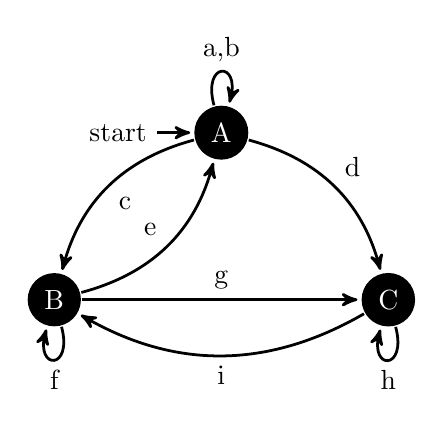
\begin{tikzpicture}[->,>=stealth',shorten >=1pt,auto,node distance=3cm,thick, line width = 1pt]
  \tikzstyle{every state}=[fill=black,draw=none,text=white,minimum size = 0.4cm]

{\node[state,initial]	(A)			{A};}
  
{\node[state]		(B) [below left of=A] 	{B};}
  
{\node[state]		(C) [below right of=A] 	{C};}


\path	(A) edge  [loop above] 	node {a,b} (A)
            edge  [bend right]	node {c} (B)
	    edge  [bend left]	node {d} (C)

        (B) edge [loop below] 	node {f} (B)
	    edge 		node {g} (C)
	    edge [bend right]	node {e} (A)
	
	(C) edge [loop below] 	node {h} (C)
	    edge [bend left] 	node {i} (B)
% 	    edge [bend left]	node {f} (A)
	 ;            
\end{tikzpicture}

%
%\caption{asdfadfs}


\caption{Robot that does a depth-first traversal of binary trees.}
\label{fig:dfs}
%\hfill
%\begin{minipage}[b]{0.45\linewidth}
%    \centering
%    \input{butterfly}
%    \caption{}
%    \label{fig: butterfly}
%\end{minipage}
%
%\begin{minipage}[b]{0.45\linewidth}
%    \centering
%    \input{eye}
%    \caption{}
%    \label{fig: eye}
%\end{minipage}
\end{figure}

% \head{Scheduling}
% Informally, a schedule $\calS$ states which agents are active at every time step.
% We need not think of the schedule as something that a centralised agent produces, but rather as a mathematical way to talk about different timing assumptions, such as synchronous, asychronous, round-robin, etc. In this work we consider asynchronous scheduling, i.e., at every 	
%
% We define typical schedules $\calS$.
%
% Let $c_0, c_1, c_2 \dots$ be a run and let $K_0, K_1, K_2 \dots$ be the active robots at each time step.
%
% The run is \emph{synchronous} if $K_n = [k]$ for every $n$.
%
% The run is \emph{asynchronous} if $|K_n| = 1$ for every $n$.
%
% The run is \emph{fair} if for every $i \leq k$ there are infinitely many $n$ such that $i \in K_n$.
%
% The run is \emph{round-robin} if $K_n = \{n \mod k\}$ for every $n$. Such runs are also fair and asynchronous.
%
% The set of runs following a schedule $\calS$ is denoted $\runs_\calS(G,\tup{R})$.
%
% \todo{formalise the fact that these schedules are definable in MSO}

% \begin{example}
% \todo{give deployment robots example. publish when you move left.}
% \end{example}

\subsection{Robot Linear Temporal Logic (\RLTL) --- a logic of tasks} \label{sec:TL}
%\head{Robot Tasks.} \label{ex:tasks}
%
%: a {\em $k$-robot task}, or simply a {\em task}, $\T$, is a function that maps a graph $G$ to a set of sequences of positions of $G$, i.e.,  $\T(G) \subseteq (V^k)^\omega$. A robot-ensemble $\tup{R}$ {\em achieves} $\T$ on $G$ if for every run $\alpha$ of $\tup{R}$ on $G$ it holds that $\alpha' \in \T(G)$, where $\alpha'$ is the sequence of positions of the run $\alpha$.
%%\sr{should define tasks to be properties of runs? i.e., include states}
%
%\item A robot {\em explores and halts} if, no matter where it starts, it a) eventually halts, and b) visits every vertex of the graph at least once.
%
%\item A robot {\em explores and returns} if, no matter where it starts, it a) eventually halts where it started, and b) visits every vertex of the graph at least once.
%Formally, $v_1 v_2 \cdots \in T(G)$ if and only if there exists $i$ such that $\{v_1,\cdots,v_i\} = V$ and for all $j \geq i$, $v_i = v_j$.
%\sr{but the robot does not know it halts. tasks should also talk about the sequence of states, not just sequence of positions?}
%\item[RT3.] A robot {\em perpetually explores} if, no matter where it starts, it visits every vertex of $G$ infinitely often.
Robots should achieve some task in their environment.
We give some examples of foundational robot tasks \cite{KKR07handbook}:

\it
\- A robot ensemble {\em deploys} or {\em reconfigures} if they move, in a collision-free way, to a certain target configuration.

\- A robot ensemble {\em gathers} if, no matter where each robot starts, there is a vertex $z$, such that eventually every robot is in $z$.

\- A robot ensemble {\em collaboratively explores} a graph if, no matter where they start, every node is eventually visited by at least one robot.

\- All of these tasks have {\em safe} variations: the robots complete their task without entering certain pre-designated ``bad'' nodes of the graph.

\ti


%
%\item[RT4.] An ensemble of robots {\em catches} a single robot if no matter where they start, at some point in time one robot in the ensemble is in the same vertex as the single robot. Note that unlike the previous examples, this task is adversarial.
% A robot {\em explores} if, no matter where it starts, it eventually visits every vertex of the graph at least once.


%no space
%Note that there are some natural relations between these tasks. If robots can explore and return, then in particular they can explore and halt. If they can explore and halt, then they can perpetually explore. If they can perpetually explore then, using the fact that they have IDs, they can gather --- every robot searches for the robot with the smallest ID, which stays still (with two agents this is called ``wait for mommy'').


%
We now define \RLTL, a logic for formally expressing tasks from the robots' points of view. The idea is that \RLTL is \LTL in which the atoms are tests.

% The syntax is \LTL over the alphabet of tests.
% The models of \RLTL are sequences of configurations. The semantics $\models_i$ (for $i \leq k$) of \RLTL are given as in \LTL, where the atomic case is
% ``robot $i$ satisfies test $\tau$ at the current configuration''. Finally, we interpret \RLTL over models of the form $\activeproj_i(\pi)$ where $i \leq k$ and $\pi \in \runs(G,\tup{R})$.


{\bf Syntax.} Let $k \in \nat$ and $\Sigma$ be a set of edge-labels.
Formulas of $\RLTL_k(\Sigma)$ are those of $\LTL(\uptau_k(\Sigma))$ where $\uptau_k(\Sigma)$ is the set of tests for $k$ robots on $\Sigma$-labeled graphs.
If $k$ and $\Sigma$ are understood from the context, we write $\RLTL$ instead of $\RLTL_k(\Sigma)$.

{\bf Semantics.} Fix $i \leq k$. For a sequence of configurations $\alpha = c_0 c_1 \cdots$ and an $\RLTL_k(\Sigma)$ formula $\varphi$, write
$\alpha \models_i \varphi$ if $\alpha$ satisfies $\varphi$ as an \LTL formula whose atoms are tests interpreted wrt robot $i$.
Formally, for formula $\varphi$ and $n \geq 0$, define $(\alpha,n) \models_i \varphi$ inductively (all cases are like \LTL, the only difference is
the first item, i.e., the atomic case):
	\it
	\- $(\alpha,n) \models_i \tau$ iff $Sat(\alpha_n,\tau,i)$ (i.e., robot $i$ satisfies test $\tau$ in $\alpha_n$);
	\- $(\alpha,n) \models_i \varphi_1 \wedge \varphi_2$ iff $(\alpha,n) \models \varphi_j$ for $j = 1,2$;
	\-	$(\alpha,n) \models_i \neg \varphi$ iff it is not the case that $(\alpha,n) \models \varphi$;
	\-  $(\alpha,n) \models_i \nextX \varphi$ iff $(\alpha,n+1) \models \varphi$;
	\- $(\alpha,n) \models_i \varphi_1 \until \varphi_2$ iff there exists $j \geq n$ such that $(\alpha,j) \models_i \varphi_2$ and for all $l \leq j < n$, $(\alpha,l) \models_i \varphi_1$.
	\ti
	Write $\alpha \models_i \varphi$ if $(\alpha,0) \models_i \varphi$.

For a $\Sigma$-graph $G$ and a $k$-robot ensemble $\tup{R}$, write $(G,\tup{R}) \models_i \varphi$ if for all $\pi \in \runs(G,\tup{R})$,
it holds that $\activeproj_i(\pi) \models_i \varphi$. We say that \emph{Robot $i$ satisfies $\varphi$}.
Finally, given \RLTL formulas $\varphi_i$ for each robot $i \in [k]$, write $(G,\tup{R}) \models \tpl{\varphi_1,\cdots,\varphi_k}$ if $(G,\tup{R}) \models_i \varphi_i$ for all $i \in [k]$.



%To express that some run satisfies $\varphi$, we could write $(G,\tup{R}) \not \models \neg \varphi$.

%Thus, given a graph $G$ and $k$-ensemble of robots $\tup{R}$ where the $i$th robot $R_i$ has state set $Q_i$, initial-state set $I_i$,
%% repeating-state set $A$,
%and halting-state set $H_i$, accepting-state set $A_i$,

\begin{example}[avoid halting state]
The \RLTL safety formula $\always  (st_{cur} \not \in H)$ says that the last published state of the robot is never in the set $H$.
\end{example}

\begin{example}[gather]
The \RLTL formula 
\[ \eventually\left[ (\bigwedge_j \VARpos_{cur} = \VARbcpos_j) \wedge \always (\VARpos_{cur} = \nextX \VARpos_{cur})\right] 
\]
 states that eventually
the current position of the robot is equal to the last published position of all the robots (including itself), and that from that point on the robot never moves.
In words, every robot satisfies this formula if and only if the robots gather (and do not disperse) at a vertex of the graph at which they last published. %sent their last broadcast.
\end{example}
%The \RLTL safety formula $\always \textsc{diff}$ where $\textsc{diff} := \bigwedge_{i \neq j} x_i \neq x_j$ says that it is always the case that the published positions of different robots do not agree. Thus, if a robot broadcasts its position whenever it moves, then this formula says that the robots never collide.

\begin{example}[deploy to leaves] \label{ex:RLTL-deploy}
 Suppose $G$ is a tree and let $\isleaf(z)$ be the test that says that position $z$ is a leaf in the tree.
%  , e.g., for binary trees,
%  $\isleaf(z) = \neg \exists x.\lambda(z,x) = lc \vee \lambda(z,x) = rc$.
 Let $\mathit{diff}$ be the formula $\bigwedge_{i \neq j} pos_i \neq pos_j$.
The \RLTL formula $\mathit{diff} \limp\left[\eventually \isleaf(\VARpos_{cur}) \wedge \always(\bigwedge_{j\neq i} \VARpos_{cur} \neq pos_j)\right]$
states that if the robots begin in different vertices of the tree $G$, then
eventually the robot reaches a leaf, and it is never in the same position as a published position of another robot.
In words, every robot satisfies this formula if and only if, assuming robots begin at different vertices of the tree $G$, the robots deploy to the leaves while not colliding with the last published positions of any other robot.
%
% In words, every robot satisfies this formula if and only if, assuming robots begin at different vertices of the tree $G$, the robots deploy to the leaves while not colliding with any other robot (according to published positions).
%
\end{example}

In order to define collaborative exploration, we will need an extension of our logic to allow tests over the accumulated positions, see Section~\ref{sec:extensions}.


%\item The $\msol$-formula $\forall \tup{x} \exists \tup{y} \exists \tup{X}. \bigcup X_i = V \wedge \psi_\alpha(\tup{X},\tup{x},\tup{y})$ says that, no matter where they start, there is a run according to a schedule that follows $\alpha$ in which the robots collaboratively explore the graph.

%\item The $\msol$-formula (to be interpreted on trees)
%where $\textsc{nonleaf}(\tup{x})$ is an $\msol$-formula expressing that every $x_i$ is not a leaf, $\textsc{leaf}(\tup{y})$ expresses that every $y_i$ is a leaf, and $\textsc{diff}(\tup{z})$ expresses that $z_i \neq z_j$ for $i \neq j$. On trees this formula expresses that for every ordering $\alpha$ of processes that switch $N$-times, there is a run according to a schedule that follows $\alpha$ such that the robots reconfigure from different internal nodes to different internal leaves.\footnote{If one wants to add that the paths of the robots are collision-free one can replace $Reach$, for the case of two robots in which robot $1$ moves and then robot $2$ moves (for instance), by the formula
%$\exists \tup{Z} \exists \tup{Y} \exists \tup{z}\left[ \psi_1(\tup{Z},\tup{x},\tup{z}) \wedge \psi_2(\tup{Y},\tup{z},\tup{y})
%  \wedge Z_1 \cap Y_2 = \emptyset \right]
%$.}

% expresses, on trees, that no matter which internal nodes of the tree two robots start on, they have a collision-free path ($Z_1 \cap Y_2 = \emptyset$) in which they reach different leaves, according to a schedule in which robot $1$ is scheduled and then robot $2$ is scheduled. Similar more complex formulas can express the reconfiguration task of Example \ref{ex:recon} for (collaborative or adversarial) $b$-switching schedules.
%\item The atomic formula $Infty(X,x,y)$ expresses that the robot, starting in position $x$, visits position $y$ infinitely often, and the set of vertices the robot visits along this run is exactly $X$. Thus $\forall x Infty(V,x,x)$ is an \RLTL\ formula expressing that the robot ``perpetually explores'' the graph.

%\item The \RLTL\ formula $\exists \tup{x} \exists \tup{X} [Halt(\tup{X},\tup{x},\tup{x}) \wedge \cup_i X_i = V ]$, which talks about $k$ robots, expresses that each robot eventually returns and halts in its starting position, and every vertex of the graph is visited by at least one of the robots.


%\item The atomic formula $Infty(X,x,y)$ expresses that the robot, starting in position $x$, visits position $y$ infinitely often, and the set of vertices the robot visits along this run is exactly $X$. Thus $\forall x Infty(V,x,x)$ is an \RLTL\ formula expressing that the robot ``perpetually explores'' the graph.

%\item The \RLTL\ formula $\exists \tup{x} \exists \tup{X} [Halt(\tup{X},\tup{x},\tup{x}) \wedge \cup_i X_i = V ]$, which talks about $k$ robots, expresses that each robot eventually returns and halts in its starting position, and every vertex of the graph is visited by at least one of the robots.

%if $k=1$ and Lemma~\ref{lem:kcompile} if $k > 1$;
%$Q := \prod_{i \in [k]} Q_i$ is the set of tuples of states, $I := \prod_{i \in [k]} I_i$ is the set of tuples of initial states, $A := \prod_{i \in [k]} A_i$ are the repeating tuples, and $H := \prod_{i\leq k} H_i$ are the halting tuples.  We will often supress mention of $k$ and write, for instance, $Reach(\tup{X},\tup{x},\tup{y})$.

%an execution $\alpha \in (V^k \times \prod_{i \in [k]} Q_i)^*$ with $\alpha_1$ an initial configuration suppose $I_i \subseteq Q_i$ are the initial states, $A_i \subseteq Q_i$ are the accepting states, and $H_i \subseteq Q_i$ are the halting states:
%$(G,\tup{R}) \models Reach(\tup{x},\tup{y})$ iff there exists a  &\textrm{ iff } \alpha_1 = (\tup{q},\tup{x}) \textrm{ is initial, and } \exists i \in \nat\, \alpha_i = \tup{y}$


% such and every $k$-robot ensemble $\tup{R} = \tpl{R_1,\cdots,R_k}$, and all $k$-tuples of states $\tup{q},\tup{s} \in \prod_{i \in [k]} Q_i$, there is an atomic formula $\tup{R}_{\tup{p},\tup{q}}$  (of arity $2k$) where $\tup{R}_{\tup{p},\tup{q}}(\tup{x},\tup{y})$ expresses that there is an execution of the ensemble $\tup{R}$ starting with configuration $\tpl{\tup{x},\tup{p}}$ and containing\sr{ending?} the configuration $\tpl{\tup{y},\tup{q}}$.


%Formulas written in MSOL can quantify over sets (of vertices and edges). Thus they can express graph properties such as whether the graph is connected, whether it has  a $k$-colouring, whether it is planar, but not whether it is rigid.\sr{are these relevant properties?}

%A cornerstone of automata theory states that MSOL over finite/infinite words/trees coincides with automata operating on finite/infinite words/trees \cite{}.
%MSOL


\section{Parameterised Verification of Robot Systems}

In this short section, we formalise the parameterised verification problem (PVP) for robot protocols and provide the basic tools which allows one to prove undecidability of certain classes of PVP problems. We illustrate with a simple undecidability result that says that PVP is undecidable, even for a single robot, on grids. In the following two sections we provide deeper undecidability and decidability results.
%, show that it is undecidable already in some very restricted cases, and then describe a simple restriction on the orderings, namely bounded switching, that guarantees decidability, which we show by reducing to the validity problem of certain logics.
%
%\head{The Parameterised Verification Problem.}

% Fix a set of $\Sigma$-graphs $\gclass$.
% \begin{definition}
% The \textbf{parameterised verification problem} $\PVP(\gclass)$ is: given a number $k \in \nat$ of robots, a $k$-robot ensemble $\tup{R}$, and an \RLTL formula $\T$, decide whether for every graph $G \in \gclass$, $(G,\tup{R}) \models \T$.
% \end{definition}
\begin{definition}
Fix a set of $\Sigma$-graphs $\gclass$, positive integer $k$, a set  $\rclass$ of $k$-robot ensembles, and a set $\tclass$ of $\RLTL_k(\Sigma)$ formulas.
The \textbf{parameterised verification problem} $\PVP(\gclass,k,\rclass,\tclass)$ is the following decision problem: given a $k$-robot ensemble $\tup{R} \in \rclass$, and a $k$-tuple of \RLTL formulas $\tpl{\varphi_1,\cdots,\varphi_k}$ from $\tclass$, decide whether for every graph $G \in \gclass$ it holds that $(G,\tup{R}) \models \tpl{\varphi_1,\cdots,\varphi_k}$, i.e., whether for every $G \in \gclass$ every robot $i$ satisfies $\varphi_i$.
\end{definition}

% \emph{Notation.}
% \it
% \- In case $\tclass$ consists of a single formula $\T$ we write $\PVP(\gclass,k,\rclass,\T)$ instead.
%
% % \- We may write $\PVP$ instead of $\PVP(\gclass,k,\rclass,\tclass)$ to ease the reading.
% \ti


% \begin{example} \sr{ordering}
% Let $\gclass$ be the set of all binary trees, $\rclass$ be the set of all $k$-robot ensembles,  let $\Omega_b := \{\alpha \in [k]^* : ||\alpha|| = b\}$ be the set of {\em $b$-switch orderings}, and let $T$ be the task expressing that if the robots start on different internal nodes of a tree then they eventually reconfigure themselves to be on different leaves of the tree, no matter which ordering from $\Omega_b$ is chosen (cf. Example~\ref{ex:formulas}). We will see later that one can decide $\PVP_{\T,\Omega_b}(\gclass,\rclass)$ given $b \in \nat$. So, one can decide, given $b$, whether the protocol from the reconfiguration example (in the Introduction) succeeds for every ordering with $b$ switches.
% \end{example}

We now introduce two-counter machines, a Turing-complete model of computation that will be used in the undecidability proofs.




\subsection{Two-counter machines}
An \emph{input-free two-counter machine} (2CM)~\cite{Minsky67} is a deterministic program manipulating two non-negative integer counters, called Counter $1$ and Counter $2$, both initialised to zero, using commands that can increment a given counter by $1$, decrement a given counter by $1$ (if the counter is not zero), and branch depending on whether or not a given counter is equal to zero. We refer to the ``line numbers'' of the program code as the ``states'' of the machine.

\begin{definition}[2CM]
A 2CM is a tuple $M = (Q,q_0,h,C)$ where $Q = [m]$ is a finite set of numbered \emph{states} ($m \in \nat$), $q_0 \in Q$ is the \emph{initial state}, 
$h \in Q$ is the \emph{halting state}, and
$C$ is a function associating each state $q \in Q$ to a \emph{command} which is an expression of the form ``increment counter $i$ and goto state $q+1$'', ``decrement counter $i$ and goto state $q+1$'', and ``if counter $i$ is zero goto $q'$ else goto $q''$'' where $i = 1,2$ and $q',q'' \in L$.
\end{definition}

We assume that every command ``decrement counter $i$'' is guarded by a command that tests that counter $i$ is not zero.
A \emph{configuration of $M$} is a triple $(q,c_1,c_2) \in Q \times \nat \times \nat$. The \emph{initial configuration} of $M$ is $(q_0,0,0)$ and the \emph{halting configurations} of $M$ are $\{h\} \times \nat \times \nat$.  Given a configuration $(q,c_1,c_2)$ there is at most one \emph{successive configuration}, i.e., if the command at $q$ is ``increment counter $1$'' then the successive configuration is $(q+1,c_1+1,c_2)$, if it is ``decrement counter $1$'' then it is $(q+1,c_1-1,c_2)$, if it is ``if counter $1$ is zero goto $q'$ else goto $q''$`` then it is $(q',c_1,c_2)$ if $c_1 = 0$ and $(q'',c_1,c_2)$ otherwise, and similar definitions hold for counter $2$. Thus, there is a unique maximal (possibly finite) sequence that starts in the initial configuration and stops once, if at all, a halting configuration is reached. This is called the \emph{computation} of the 2CM. We say that the 2CM \emph{halts} if the computation is finite and ends in a halting configuration.
% Observe that if the computation is finite then the values of both counters are bounded by some integer $n$. 
The \emph{non-halting problem for 2CMs} is to decide, given a 2CM $\cm$, whether it does not halt. This problem is undecidable (cf. \cite{Minsky67}), and is usually a convenient choice for proving undecidability of problems concerning parameterised systems due to the simplicity of the operations of counter machines~\cite{Emerso03,AJKR14,DBLP:conf/cade/AminofR16}.

\subsection{Basic undecidability result}
To show undecidability we reduce the non-halting problem of two-counter machines to certain parameterised verification problems.

That is, given a 2CM machine $M$, we build robot(s) $\tup{R}$ and a tuple of formulas $\tpl{\varphi_1,\cdots,\varphi_k}$
such that the run of $M$ never reaches a halting state if and only if
$(G,\tup{R}) \models \tpl{\varphi_1,\cdots,\varphi_k}$ for all $G \in \gclass$. We illustrate with a basic undecidability result on grids that states that
PVP is undecidable already for a single robot on grids with simple testing abilities and a safety task.
The proof ideas were already observed in \cite{BlHe67} for a different setting.
% for ``2-dimensional automata''.


\begin{theorem}[Grid, boundary testing] \label{thm:undec-1robotgrid}
$\PVP(\gclass,k,\rclass,\tclass)$ is undecidable for the following data:
\it
\- $\gclass = \{G_n : n \in \nat\}$ is the set of grids (so $\Sigma = \{u,d,l,r\}$),
\- $k = 1$,
\- $\rclass$ is the set of $1$-robot ensembles, with no publishing states, that can test whether or not they are on a given boundary of the grid,
\- $\tclass$ consists of the single safety formula $\always (st_{cur}  \neq h)$.
\ti
\end{theorem}



% \todo{- add to statement of thm that robots don't need publishing states.}

% \todo{- fix initial states. either put them in the formula, or in the graph.}
\begin{proof}
 The idea is that counter values $(n,m) \in \nat^2$ are encoded by the robot being at position $(n,m)$ of the grid, and the only tests that are needed are to check whether or not the robot is on a given boundary. Indeed, given a 2CM $\cm$, the robot $R_\cm$ stores the current state of $\cm$. If the current state is $q$ and the current command is ``increment (resp. decrement) counter $1$'' then the robot tests if it is on the right (resp. left) boundary, and if not it moves one step to the right (resp. left) and updates its state to $q+1$, and if yes it enters a failure sink state $\bot$. ``Increment (resp. decrement) counter $2$'' is similar, and involves moving up (resp. down) and entering the failure sink $\bot$ if the tests fail. Finally ``test counter $1$ (resp. $2$) for zero'' is done by testing if the robot is on the left (resp. bottom) boundary. Before the robot starts the simulation, it moves to co-ordinate $(0,0)$ (which it can do since it can test for boundaries). Note that for every $n$ the set $\runs(G_n,R_\cm)$ contains a single run. Moreover, the run of $\cm$ never halts iff for every $n$ the run in $\runs(G_n,R_\cm)$ never reaches the halting state. \qed
\end{proof}

This theorem strongly suggests that one cannot get decidable PVP unless one limits at least one of the following: the testing abilities of the robots, the moving abilities of the robots, or the class of graphs. The above undecidability result for grids made use of only a single robot with very basic testing abilities (i.e., boundary detection). Thus, there is not much hope for an interesting model if we further restrict the testing abilities. Limiting the movement of robots on grids was studied in \cite{AAMAS16Grids}. There, one disallows robots from specifying their exact positions in the grid, e.g., a robot may decide to move to the left but not specify the exact number of steps. In the present work, instead, we consider robots with powerful remote-testing and the ability to specify their movements exactly. We restrict the set of graphs that are definable in monadic second-order logic and of bounded clique-width. We call these \courcellian sets of graphs. These do not include grids, but do include, e.g., lines, trees, and cliques, see section~\ref{sec:dec}.
% As we will see in Section~\ref{sec:DEC k=1} this restriction on the sets of graphs is enough to get decidable PVP for systems consisting of only a single robot.
However, this restriction on its own is not enough.
In the next section, we give undecidability results for multiple robots and possibly the simplest sets of \courcellian graphs, i.e.,
lines (thus indicating that further restricting the graphs will not yield interesting models).
The undecidability results imply that one has to impose limitations on their
``communications'' in order to regain decidability for multiple robots.
Specifically, the limitation on the robots state that there
is a bound on the number of times that a robot can test another robot's current
state and position, and a similar limitation must
be imposed on the specification logic.
%Interestingly enough, these restrictions are neccessary even if one limits robots to very basic tests (i.e., collision detection).

% \ba{Update rest of this section.}
%
%
% In the next section it is shown that the PVP is undecidable for two synchronous robots on a line, and very simple tasks. In light of this negative result, we explore in what ways we can restrict the robots to gain decidability. One possible direction is to limit the sensing/communication between the robots. Indeed, the above mentioned undecidability result assumes that each robot can sense/query whether the other robot is at the left-most position of the line. Another possibility is to consider the case of asynchronous robots. In Section \ref{sec:PVPundec} we show that the assumption of asynchronous robots alone does not guarantee decidability of the parameterised verification problem already in the very restricted case of reachability tasks on lines. Interestingly enough, our proof also applies \todo{check} to the synchronous case,  and assumes only very limited sensing capabilities, namely, that a robot can sense which of the other robots shares the same position with it (i.e., ``collision detection''). This fact strongly suggests that limiting the robots' sensing capabilities may not be a very fruitful direction. In Section \ref{sec:PVPdec} we show that for asynchronous robots with full testing abilities we can guarantee decidability by i) restricting to context-free environments, and ii) restricting to $B$-broadcast schedules. As we have just seen, dropping either of these two restrictions results in undecidability.



\section{Decision Procedures} \label{sec:decision procedures}



\begin{theorem}
 NE-emptiness of $\LEX(\LTL,\mp)$-games is decidable. \todo{Todos: 1) debug, 2) polish, 3) calculate complexity of the algorithm}
\end{theorem}

\begin{proof}[Sketch]
We prove this in three steps. In the first step we push the weights of $G$ into the states and translate the result into a $\LEX(\parity,\mp)$ game $G'$ such that $\NE(G) = \NE(G')$. Here $\parity$ is an aggregation function that maps a sequence of priorities (integer weights) to $0$ if the smallest priority occuring infinitely often is even, and to $1$ otherwise (the priorities are given as a second weight function, in addition to $\kappa$). In the second step we show how to reduce $NE$-emptiness of $G'$ 
to the problem of solving two-player zero-sum games $H$ in which player $0$ has a $\LEX(\parity,\mp)$ objective. We do this by adapting the proof that shows how to decide $NE$-emptiness of mean-payoff games~\cite{DBLP:conf/concur/UmmelsW11}.  In the third step we reduce $H$ to solving mean-payoff parity games. These are two-player zero-sum games in which the objective of player $0$ is to ensure both the parity condition holds and that the mean-payoff is maximised~\cite{DBLP:conf/lics/ChatterjeeHJ05}. Formally: the payoff is $-\infty$ if the smallest priority occuring infinitely often is even, otherwise it is the mean-payoff of the weights.

% $\parity(\alpha) \in \{0,1\}$ is $0$ iff the $min(inf(\alpha))$ is even, where $inf(\alpha)$ consists of the weights occuring infinitely often in $\alpha$.

\head{Replace \LTL by Parity}
For the first step, push the weights to the states. This is done by replacing $St$ by $St \times Act^{Ag}$ and defining the weight of $(s,d)$ to be $\kappa(d)$. Convert each \LTL formula $\varphi_a$ into a deterministic parity automaton $D_a$ of size double-exponential in $\varphi_a$~\cite{??}. To build the game $G'$ form the product weighted arena $\St' = \St \times \prod_a D_a$. Each agent has a pair of weights associated with each state, i.e., a priority (coming from $D_a$) and the integer weight (coming from $\kappa$).  Given a play, the payoff for an agent is $(x,y)$ where $x = 0$ iff the smallest priority occuring infinitely often on the play is even, and $y$ is the meanpayoff of the integer weights. By construction we have that $\NE(G) = \NE(G')$.

\head{Reduce \NE\ to path-finding}
For the second step, we adapt the proof in Section~6 of \cite{DBLP:conf/concur/UmmelsW11} that shows how to decide $NE$-emptiness for mean-payoff games. For $a \in Ag$ and $s \in \St$ define the \emph{punishing value} $p_a(s)$ to be the $\lex$-largest $(x,y)$ that player $a$ can achieve from state $s$ by ``going it alone'', i.e., by playing against the coalition $Ag \setminus \{a\}$.  We will show how to compute these values in the third step. 

Definition: For an agent $a$ and $\bar{z} \in \mathbb{R}^{|Ag|}$, a pair $(s,d) \in \St \times Act^{Ag}$ is \emph{$\bar{z}$-secure for $a$} if $p_a(tr(s,d')) \leq z_a$ for every $d' \in Act^{Ag}$ that agrees with $d$ except possibly at $a$. 

Claim: $\NE(G')$ is non-empty iff there exists $\bar{z}$ where $z_a \in \{p_a(s) : s \in \St\}$ and there exists an execution $\pi = s_0 d_0 s_1 d_1 \cdots$ in $G'$ such that for every agent $a$,  i) $z_a \leq pay_a(\pi)$ and ii) for all $i \in \mathbb{N}$, the pair $(s_i,d_i)$ is $\bar{z}$-secure for $a$. 


Sketch proof of Claim: Suppose $\NE(G')$ is non-empty. Let $\pi$ be the execution resulting from some Nash-profile. 
Let $z_a = \max\{p_a(\delta(s_n,d'_n)) : n \in \mathbb{N}, \wedge_{b \neq a} d'_n(b) = d_n(b)\}$, i.e., $z_a$ is the largest value player $a$ can get by deviating from $\pi$. Clearly $(s_n,d_n)$ is $\tup{z}$-secure for $a$. Moreover, $z_a \leq pay_a(\pi)$: indeed, if $z_a = p_a(\delta(s_n,d'_n)) > pay_a(\pi)$ then player $a$ would deviate at step $n$ by playing $d'_n$ and achieve a higher payoff, contradicting the choice of $\pi$ as the execution of a Nash-profile.

For the converse direction, let $\bar{z}$ and $\pi$ be given with the stated properties. The following is a Nash-profile: every agent plays ``follow $\pi$'' until, and if, a single player, say $a$, deviates, say at state $s$; in that case the other agents play a punishing strategy, i.e., a strategy that ensures player $a$ achieves no more than he possibly can given the current history. It can be shown that this value is $p_a(s)$ for $LEX(\parity,\mp)$ payoff functions (since such payoff functions are prefix-independent). This completes the proof of the claim.





Note that $p_a(s)$ is the value of the two-player zero-sum game $H_a(s)$ in which the first player is trying to maximise $a$'s lexicographic payoff $pay_a(\cdot)$ and the second player is adversarial (i.e., trying to minimise $pay_a(\cdot)$). 
Thus, we have 
reduced $NE$-emptiness of $\LEX(\parity,\mp)$ games to the problem of computing the values of these games $H_a(s)$. 

\head{Reduce to solving mean-payoff parity games} 
In the third and final step we show how to reduce the games $H = H_a(s)$ to solving mean-payoff parity games. We consider two games $J$ and $K$, both on the same weighted arena as $H$, but with different objectives: the first player's objective in $J$ is the mean-payoff parity objective, and the first player's objective in $K$ is the mean-payoff objective. Let $j$ be the value of $J$ and $k$ the value of $K$. It is easy to see that the value of $H$ is $(1,j)$ if $j \neq -\infty$ and $(0,k)$ otherwise.
\end{proof}

\begin{theorem}
 E-NASH of $\LEX(\LTL,\mp)$-games is decidable. 
\end{theorem}
\begin{proof}
Check that previous works with: $\NE(G') \subseteq \Phi$ iff there exists $\bar{z}$ where $z_a \in \{p_a(s) : s \in \St\}$ and there exists an execution 
$s_0 d_0 s_1 d_1 \cdots$ in $G'$ \textbf{satisfying $\Phi$} such that each transition $tr(s_i,d_i) = s_{i+1}$ (for $i < \omega$) is $\bar{z}$-secure. 
\end{proof}



\section{Related Work}

NE-emptiness is the main decision problem studied in this paper, i.e., decide if a given multiplayer concurrent game has a Nash Equilibrium or not. 
We studied this problem for $\LEX(\LTL,\mp)$-games, i.e., graph-games in which agents are trying to maximise their lexicographic payoff whose first co-ordinate is an \LTL formula and whose second co-ordinate is the mean-payoff of its weights. We proved the problem is $2$\exptime-complete.

\head{Other objectives}
NE-emptiness has been studied for graph-games with other objectives, a sample of which are given in Table~\ref{tab:NE-emptiness}.
\begin{table}\label{tab:NE-emptiness}
\begin{center} 
\begin{tabular}{llll}
Objectives			& Complexity 			& Reference\\
\hline
$\LEX(\LTL,\mp)$		& $2$\exptime-complete		& This paper\\
\LTL 				& $2$\exptime-complete		& \cite{DBLP:journals/tocl/MogaveroMPV14}\\
mean-payoff (\mp)			& \np-complete			& \cite{DBLP:journals/corr/abs-1109-6220}\\
reachability			& \np-complete			& \cite{DBLP:journals/corr/BouyerBMU15}\\
lexicographic reachability	& \pspace-complete		& \cite{DBLP:journals/corr/BouyerBMU15}\\
B\"uchi				& \ptime-complete		& \cite{DBLP:journals/corr/BouyerBMU15}\\
lexicographic B\"uchi		& \ptime-hard, in \np		& \cite{DBLP:journals/corr/BouyerBMU15}\\
% counting ???		& ???				& \cite{DBLP:journals/corr/BouyerBMU15}
% parity			& ${\sf P}^\np_{||}$-complete	& \cite{DBLP:journals/corr/BouyerBMU15}\\
\end{tabular}
\caption{Complexity of NE-emptiness for multiplayer concurrent-games with objectives from various classes.}
\end{center}
\end{table}
$\LEX(\LTL,\mp)$ generalises both mean-payoff games (simply set every formula to be $\true$) and \LTL games (simply set all the weights of the arena to be $0$). That NE-emptiness is decidable in $2$\exptime for \LTL games follows from a more general result, i.e., that model checking \emph{strategy logic} on concurrent game structures (i.e., arenas without the weights) is decidable \cite{DBLP:journals/tocl/MogaveroMPV14}. To get the $2$\exptime upper bound one writes the existence of a NE in a fragment of strategy logic (i.e., nested-goal with alternation number $1$) whose model checking problem is decidable in $2$\exptime. We cannot apply strategy logic to $\LEX(\LTL,\mp)$ games since the latter have a quantitative component while strategy logic, being built on top of \LTL, can only express qualitative objectives. 
Instead, as discussed in Section~\ref{sec:decision procedures}, we generalised the proof in~\cite{DBLP:journals/corr/abs-1109-6220} of the fact that NE-emptiness is in \np\ for mean-payoff games. 

We remark that the hardness results for lexicographic reachability and lexicographic B\"uchi are for lexicographic orders on an arbitrary (but finite) number of co-ordinates.

\head{Turn-based}
Very simple concurrent games, such as matching pennies, do not have NE. However, there are many classes of turn-based graph-games that always have NE. For instance, turn-based mean-payoff games~\cite{Alpe91}, turn-based games with $\omega$-regular objectives (which include \LTL objectives)~\cite{CJM04}, turn-based quantitative-reachability games~\cite{Brihaye2013}. Actually, this phenonemon has a general explanation: under certain conditions the existence of (finite-memory) NE for a class of objectives follows from the (finite-memory) determinacy of two-player zero-sum games with those objectives~\cite{DBLP:journals/corr/0001P16,Brihaye2013}. Although the latter citations do not cover the case of turn-based $\LEX(\LTL,\mp)$-games, we use a similar strategy in Theorem~\ref{thm:TB} to prove that these too always have NE. Determinacy (and the complexity of determining the winner) of two-player zero-sum games has been studied for a variety of objectives, 
i.e., mean-payoff~\cite{EM79,ZwPa95}, $\omega$-regular (which include $\LTL$-objectives)~\cite{DBLP:conf/dagstuhl/2001automata}.
%In addition, there are various uniform explanations for when such zero-sum games have positional or finite-memory winning strategies~\cite{Demri?,AmRu14,halfpositional}.

\head{Randomised Strategies}
We have considered deterministic strategies. Randomised strategies are functions that map a history to a probability distribution over actions. 
NE-emptiness is undecidable for randomised strategies on games with reachability objectives for each player~\cite{DBLP:conf/fsttcs/BouyerMS14}. Since reachability objectives are a special case of $\LEX(\LTL,\mp)$ objectives, we have undecidability of NE-emptiness for randomised strategies on $\LEX(\LTL,\mp)$ games.

\todo{IMPORTANT RELATED WORK THAT NEEDS TO BE SUMMARISED: cite{DBLP:journals/corr/abs-1303-0789}; as well as work on secure-Equilibria}

% \head{Other representations of games}
% Nash's famous result states that every finite game in strategic form has a randomised NE~\cite{??}. Computing such a NE is complete for the complexity class PPAD \cite{DBLP:journals/siamcomp/DaskalakisGP09}.\todo{check}
% 
% \todo{Stochastic games...}



 
% \begin{theorem} \cite{DBLP:journals/corr/abs-1109-6220}
%  The following problem is NP-complete: given $\bar{x} \leq \bar{z} \in \mathbb{Q}^{|Ag|}$ and a mean-payoff game, decide if there is a
%  NE, say with payoff $\bar{y}$, that satisfies $\bar{x} \leq \bar{y} \leq \bar{z}$.
%  \end{theorem}



% 
% \head{``Pure Nash Equilibria in Concurrent Deterministic Games'', Bouyer et al. \cite{DBLP:journals/corr/BouyerBMU15}}
% 
% The paper then gives the exact complexity of NE-emptiness for many $\omega$-regular 
% objectives, and semi-quantitative versions of these (like counting or 
% lexicographic). E.g., 
% \begin{theorem}[\cite{DBLP:journals/corr/BouyerBMU15}]
% The complexity of NE-emptiness  for:
% \begin{enumerate}
%  \item reachability- and safety-games are $\np$-complete, 
%  \item Buchi-games are $\ptime$-complete,
%  \item parity-games is ${\sf P}^\np_{||}$-complete,
%  \item Muller-games is $\pspace$-complete,
%  \item lexicographic Buchi-games are in $\np$.
% \end{enumerate}
% \end{theorem}

% \head{  Synthesis from LTL Specifications with Mean-Payoff Objectives`` \cite{DBLP:journals/corr/abs-1210-3539}}
% Two player, synthesis of specifications written in LTL with mean-payoff weights. 
% Objective is ''formula must be true and weights must be maximised``. Reduced to parity games.
% 
% \head{ A four-person chess-like game without Nash equilibria in pure stationary strategies}
% https://arxiv.org/abs/1411.0349
% 
% This paper shows that NE need not be memoryless for games in which the payoff depends on the
% first cycle formed. The example in their paper can be expressed in terms of meanpayoff.
% 
% 
% 
% \head{``Extending finite memory determinacy: General techniques and an application
%                to energy parity games'' \cite{DBLP:journals/corr/0001P16}}
%              
%              
%            Shows how to extend determinacy of win/lose games to finite-state NE of multiplayer games.
%            Turn based.
%            
%            
%       \section{OLD --- The model}


	
		\begin{definition}[CCGS]
		A \emph{$d$-dimensional Cost Concurrent Game Arena} (\CCGA) is a
		tuple $A=\tpl{\Ag, \Stt, \Act,\iota,\kappa,d}$
		\begin{enumerate} \item $\Ag$ is a finite non-empty set of \emph{agents} (we write 
			$\NElm			= \card{\Ag}$);
			\item $\Act$ is a set of the actions;
			\item $\Stt$ is a finite non-empty set of \emph{states} and $\iota$
						is the \emph{initial state};
			\item $\trn: \Stt \times \Act^{\Ag} \rightarrow \Stt$ is
						a \emph{transition function} mapping each pair consisting of a
						state and an action for each agent to a state,
			\item $d \in \nat$ is the {\em dimension} and $\kappa: \Ag \to (\Stt \times \Act^{\Ag} \rightarrow \mathbb{Z}^d)$ is a \emph{cost function}.
		\end{enumerate}
		\end{definition}


An \emph{execution} $\pi$ is an infinite sequence over $\Stt \times \Act^{\Ag}$ that
respects the transition function.  Let $\exec$ denote the set of all
executions. 

A {\em payoff function} is a function $\mu: \Ag \to (\exec \to \mathbb{R})$, i.e., it
assigns a payoff/utility to each agent.  The payoff may depend on the costs and
the states along the execution. Each agent is trying to maximise its payoff.
A \emph{$d$-dimensional Cost Concurrent Game Structure} (\CCGS) is a tuple $G = (A,\mu)$ where $A$ is a \CCGA and $\mu$ is a payoff function.
In case the payoffs are always in the set $\{0,1\}$ such games are called ``win-lose''.

A \emph{strategy profile} is a strategy for each agent. We write these as $\sigma: \Ag \to (\hist \to \Act)$ where $\hist$ is the set of finite sequences of states.
\todo{Note: we do not include actions in histories... this seems a reasonable choice for discussing NE in distributed systems}
A strategy profile $\sigma$ induces a unique execution $\pi_\sigma$.

\todo{todo: define turn-based game as a special case}

\subsection{Payoff functions}

In order to define concrete payoff functions we typically aggreggate the costs incurred for each player. 
Each execution $\pi$ induces, for each agent $i$, a sequence of costs
$c_i(\pi) \in (\mathbb{Z}^d)^\omega$. Write $c_i^j(\pi) \in \mathbb{Z}^\omega$ for the sequence of costs
for player $i$ in dimension $j \leq d$.




In what follows, the name of the classes of games (mean-payoff, parity, LTL) should really be prefixed by 
``multi-player'' so as not to cause confusion with the two-player zero-sum case.
For $\alpha \in \mathbb{Z}^\omega$, define $mp(\alpha)$ to be the long-term average of the sequence $\alpha$, i.e.,
the lim-inf of the the average of the first $n$ terms of $\alpha$.


\begin{example}[Mean-payoff games]
Let $d = 1$, and let $\mu(i)(\pi) = mp(c_i(\pi))$ be the long term average of
$c_i(\pi)$. Call these {\em mean-payoff games}.
\end{example}

  \begin{example}[$F$-mean payoff games]
  Fix a function $F:\mathbb{R}^d \to \mathbb{R}$ and define $\mu(i)(\pi) = F(mp(c_i^1(\pi)), \cdots, mp(c_i^d(\pi)))$,
  i.e., the payoff for player $i$ is the value of $F$ on the long-term averages of its costs. 
  Call such games {\em $F$-mean payoff games}. Here are some illustrative examples of functions $F$:
\begin{enumerate}
\item $F$ is a threshold function. For instance, if $d = 1$ and $F(x) = 1$ if $x > 0$ and $0$ otherwise.
Let us call these \emph{Threshold Mean-Payoff games}.
\item $F$ is the average of its arguments, 
\item $F$ is the max of its arguments,
\item $F$ counts the number of arguments that are positive,
\item $F$ is the lexicographic. For instance, if $d = 2$, define $F(x,y) = 0$ if $x \leq 0$, $1$ if $x \geq 0$, and $2$ if $x \geq 0$ and $y \geq 0$.
Call these \emph{lexicographic threshold mean-payoff games}. 
\end{enumerate}

\end{example}

We give some more examples with $d = 1$.


\begin{example}[Parity-games]
Let $d = 1$, and let $\mu(i)(\pi)$ equal $1$ if the largest cost of player $i$ seen infinitely often on $\pi$ is even, and equal to $0$ otherwise. 
Call such games {\em parity-games}. 
\end{example}

\begin{example}[Generalised Muller games]
 Let $d = 1$, and let $\mu(i)(\pi)$ depend only on the set of states that occur infinitely often in $\pi$. Call such games {\em generalised Muller-games} after that fact
 that a Muller-game is such a game in which the payoffs are from $\{0,1\}$.
\end{example}

\begin{example}[LTL-games and $\omega$-regular games]
A \emph{LTL-game} is one in which each player has an LTL objective that it is trying to satisfy. 
Formally, replace the cost function in CGCS's by state-labelings $\lambda:\Stt \to 2^{\Ap}$ over some fixed set of atoms $\Ap$.
Given $N$ LTL formulas $\phi_i, i \leq N$, the payoff for player $i$ is $1$ if $\pi \models \phi_i$ and $0$ otherwise.

More generally, if $\phi_i$ is an $\omega$-regular language (i.e., $\phi_i \subseteq (2^{\Ap})^*$) then we have \emph{$\omega$-regular games}.
\end{example}

\begin{example}[Oxford Games]
Let $d = 1$ and suppose every weight is positive. Let $\phi_i$ be \LTL formulas, one for each agent. 
An \emph{Oxford} game (because we discussed some variation of this in Oxford)
has payoff that maps a play $\pi$ to $0$ if $\pi \models \neg \phi_i$ and to $mp(c_i(\pi))$ otherwise. The goal is to maximise the payoff.
\end{example}

\note{Can we capture zero-sum mean-payoff games in which one player maximises and the other minimises?}

\section{The decision problems}

Let $\C$ be a set of games. We define two decision problems.
\begin{definition}
 \emph{E-NASH($\C$)}: Decide if a given game from $\C$ has a Nash-Equilibrium.
\end{definition}

\begin{definition}
 Memoryless-E-NASH($\C$): Decide if a given game from $\C$ has a Nash-Equilibrium made of memoryless strategies.
\end{definition}


We now discuss the relationship between some of the games.

\begin{definition}[Equivalent games]
Call two games $G,G'$ \emph{(memoryless-)equivalent} 
if for every strategy profile $\sigma$ (of memoryless strategies) in $G$ there exists a strategy profile 
$\sigma'$ (of memoryless strategies) in $G'$, and vice versa, such that $\mu(i)(\pi_\sigma) = \mu'(i)(\pi_{\sigma'})$ for each agent $i$. Here $\pi_\sigma$ and $\pi_{\sigma'}$
are the plays induced by the strategy profiles $\sigma$ and $\sigma'$ respectively.
\end{definition}

It is useful to have effective transformations of games from one class into games of another class. Indeed, if $\C,\C'$ are two classes of games for which 
there is an effective transformation of games in $\C$ into equivalent games in $\C'$ then E-NASH($\C$) can be reduced to E-NASH($\C'$). A similar statement holds for the memoryless case.

For instance, it is immediate from the definitions that every parity-game is (trivially) equivalent to a Muller game (i.e., itself), 
and every Muller game is (trivially) equivalent to an $\omega$-regular game (i.e., itself). 

Here are some more interesting equivalences. 

\begin{theorem}\label{thm:LTL to parity}
Every LTL-game can be effectively translated into an equivalent parity-game with $2$-exponential blowup. \todo{This should also work for objective-LTL games.}
\end{theorem}

\begin{proof}[Sketch]
Let $G$ be an LTL-game.
The idea (which is standard for two-player zero-sum games) 
is to convert the LTL formulas into deterministic parity-word automata (DPW), and then form the product of the original game with these automata. 
Being deterministic, the automata
simply annotate the game $G$. 

Here are some details. Translate each LTL formula $\phi_i$ into a deterministic parity-word automaton $A_i$ in which priorities are on edges 
(instead of, as usual, states). Say $A_i$ has state set $Q_i$. 
Then form the parity-game $G'$ as the product of $G$ and $\prod Q_i$. The cost for player $i$ of transition of $G'$ is defined to be the priority of the corresponding 
transition in $A_i$. Then $G$ and $G'$ are equivalent.
\end{proof}


\begin{theorem} \label{thm:PG-MP}
Every parity-game can be effectively translated into a memoryless-equivalent threshold mean-payoff game with no blowup.
\end{theorem}

\begin{proof}[Sketch]
Let $G$ be a parity-game. The idea (cf. e.g., \cite{Jurd98}) is to replace each priority $p$ by the cost $(-m)^p$ where $m$ is 
the number of states of $G$. Then, if $\pi$ is the play resulting from a memoryless-strategy profile in $G$ then the highest priority for player $i$ on $\pi$ is even 
if and only if $mp(c_i(\pi)) > 0$.
\end{proof}

%\todo{Similarly, the lexicographic payoff is a special case of $F$-mean payoff games.}

\begin{corollary}
 For every LTL-game there is a memoryless-equivalent threshold mean-payoff game with $2$-exponential blowup.
\end{corollary}

\todo{Question. Is this same true if we drop ``memoryless''?}

\begin{conjecture} \label{conj:oxford-mp}
Oxford games are memoryless-equivalent to lexicographic threshold mean-payoff games with $2$-exponential blowup.
\end{conjecture}
\begin{proof}[Sketch]
 Let $G$ be an Oxford game. Replace the LTL formulas by DPW, as in Theorem~\ref{thm:LTL to parity}. Then replace DPWs by mean-payoff condition, as in Theorem~\ref{thm:PG-MP}.
\end{proof}


%The following property is useful: a payoff function is \emph{prefix-independent} if $\mu(i)(\pi) = \mu(i)(\pi')$ for every suffix $\pi'$ of $\pi$.
%All the payoff functions above are prefix-independent, except some LTL and $\omega$-regular games.


\section{Related Work and Conjectures}

We now state some known results and sketch their proofs. For the sake of the draft, we also
conjecture some results and sketch proof-ideas.

\subsection{Concurrent Setting}
The authors in \cite{DBLP:journals/corr/BouyerBMU15} give a general reduction from multiplayer concurrent games with preference relations to two-player zero-sum games such that the former has a NE
iff the later has a winning strategy. In their words:

\begin{verbatim}
We propose a novel transformation of the multi-player
concurrent game (with a preference relation for each player) 
into a two-player zero-sum turn-based game, which we call 
the suspect game. Intuitively, in the suspect game, one of 
the players suggests a global move (one action per player 
of the original game), with the aim to progressively build 
a Nash equilibrium; while the second player aims at proving 
that what the first player proposes is not a Nash equilibrium.
This transformation can be applied to arbitrary concurrent games 
(even those with infinitely many states) and preference relations
for the players, and it has the property that there is a 
correspondence between Nash equilibria in the original game and 
winning strategies in the transformed two-player turn-based 
game. The winning condition in the suspect game of course depends 
on the preference relations of the various players in the 
original game. 
\end{verbatim}

The paper then gives the exact complexity of ENASH for many $\omega$-regular 
objectives, and semi-quantitative versions of these (like counting or 
lexicographic). E.g., 
\begin{theorem}[\cite{DBLP:journals/corr/BouyerBMU15}]
The complexity of ENASH for:
\begin{enumerate}
 \item reachability- and safety-games are $\np$-complete, 
 \item Buchi-games are $\ptime$-complete,
 \item parity-games is ${\sf P}^\np_{||}$-complete,
 \item Muller-games is $\pspace$-complete,
 \item lexicographic Buchi-games are in $\np$.
\end{enumerate}
\end{theorem}



\begin{conjecture} \label{conj:ENASH-mpgs}
E-NASH for threshold mean-payoff games is decidable in \expspace.
Memoryless E-NASH for threshold mean-payoff games is decidable in \exptime. The same statements hold for lexicographic mean-payoff games.
\end{conjecture}
\begin{proof}[Idea]
% Perhaps the suspect game can be applied, or GP's idea of reducing E-NASH to synthesis and satisfiability can be applied.
 We first sketch the proof for threshold mean-payoff games (i.e., not lexicographic).
 Given a game $G$, let $\phi_a$ denote the condition that the mean-payoff of the costs of a play for agent $a$ is greater than $0$. 
 Guess the set of losers $L \subseteq \Ag$ and consider the following turn-based two-player zero-sum game $G_L$ played on the states of $G$
 between $E$ and $A$, who alternate turns, with $E$ going first. $E$ plays tuples of actions $m$, one for each player,  
 and $A$ plays states.  There are $|\Ag|+1$ modes the game can be in: neutral or $a$-deviating for $a \in \Ag$. Before any of his moves, $A$ can decide to switch modes from neutral to $a$-deviating for some $a \in \Ag$, and once in $a$-deviating mode, the play stays in $a$-deviating mode.  Play starts from the initial state, in neutral mode. The modes are used as follows. Suppose the current state is $q$ and $E$ has chosen the tuple $m$. 
In the neutral mode $A$ plays $q' = \delta(q,m)$. In $a$-deviating mode $A$ may play $q' = \delta(q,m')$ where $m'$ agrees with $m$ except possibly on $a$'s action. A play $\pi$ is won by $E$ iff 
 $\pi \models \bigwedge_{a \in L} \neg \phi_a \wedge \bigwedge_{a \in \Ag \setminus L} \phi_a$. Then: $E$ has a (finite-memory) winning strategy in $G_L$ iff $G$ has a (finite-memory)  Nash Equilibrium whose losers are $L$.
 
 Thus, we have reduced the (memoryless) ENASH problem to solving (in memoryless strategies) exponentially-many polynomially-sized two-player zero-sum games $H$ with objective that is a boolean combination of mean-payoff thresholds. Each game $H$ is solvable for arbitrary strategies \expspace (using Petri-Nets). So the whole procedure can be done in \expspace.
 Each game $H$ is solvable for memoryless strategies in \exptime (just run through all the memoryless strategies, and look for a lasso satisfying the winning condition). So the whole procedure can be done in \exptime.
 
 To get the result for the lexicographic case, adapt the formula that $E$ needs to satisfy to reflect the lexicographic order on the threshold objectives.
\end{proof}
The complexity can probably be improved. Use nondeterminism to guess $L$, and then solve a single game $H$. It is known that if the boolean combination of the objectives is a conjunction of ``greater-than'' conditions, then the complexity is co-\np-complete for finite-strategies, and \np-complete for memoryless strategies~\cite{DBLP:conf/fsttcs/ChatterjeeDHR10}. 

 \begin{conjecture}
  Memoryless-ENASH for Oxford-games is decidable in 3\exptime.
 \end{conjecture}
\begin{proof}[Sketch]
 By Conjecture~\ref{conj:oxford-mp}, we can reduce the problem to Memoryless-ENASH of lexicographic threshold mean-payoff games. By Conjecture~\ref{conj:ENASH-mpgs}
 these can be solved in \exptime.
\end{proof}

\todo{Q: What about a lower bound? See \cite{DBLP:journals/corr/BouyerBMU15}}


% The following is folklore: one can decide if a given player in a two-player 
% concurrent game has a winning strategy by reducing to a turn-based game in which 
% that player always moves first.

\subsection{Turn-based Setting}

The first paper studies mean-payoff games.

\begin{theorem}[\cite{Alpe91}] \label{thm:turnbased:MP}
In turn-based mean-payoff games:
\begin{enumerate}
 \item Memoryless NE may not exist if $N > 2$, \todo{Q: what about $N \leq 2$?}
 \item Finite-state NE exist, and the number of states may be taken to be $|\Stt|!$. \todo{Q: can this be improved to memoryless?}
\end{enumerate}
\end{theorem}
\begin{proof}[Sketch]
The main part of the proof of 2. is to show that such games are equivalent to certain 
finite-duration games: play as usual, but stop once a state is repeated and a 
simple cycle is formed, and define the utility of the play for agent $i$ to be 
mean-payoff costs of the cycle.  Given this, use backward induction (i.e., 
Zermelo-Kuhn theorem) to deduce that the finite duration game (and hence the 
original CCGS) admits a NE. Each strategy needs to remember at most the ordering 
of the states as they are encountered, i.e., $|\St|!$ memory is enough. This 
bound on the strategies of the finite-duration game transfers to the original 
game. 
\end{proof}

The next paper studies multi-player stochastic games with $\omega$-regular objectives.
Deterministic games are a special case.

\begin{theorem}[special case of \cite{CJM04}]
Turn-based games with prefix-independent $\omega$-regular objectives have
finite-state NE. \todo{Check if for parity objectives memoryless strategies suffice}
\todo{Check if paper mentions prefix-independent}
\end{theorem}
\begin{proof}[Sketch] 
The idea is that a NE is one where the players play to try and achieve their 
own 
objectives, but the moment a player deviates all the others punish that player 
by ensuring she still can't achieve her objective if she couldn't in the first 
place.

In more detail, let $W_i$ be the 
winning region of the game in which player $i$ tries to achieve its objective 
and all the others form an adversarial-coalition. This is a two-player zero-sum 
game (i.e., player $i$ vs a single player representing all the other players, 
called the adversarial coalition) with $\omega$-regular objective. These games 
are determined, and thus the states $L_i$ not in $W_i$ are won by the 
adversarial coalition. Let $\sigma_i$ be a strategy for player $i$ that wins 
from $W_i$, and let $\sigma_i^j$ be a strategy for players $j \neq i$ such that 
they, collectively, ensure that player $i$ loses on $L_i$. Define a strategy 
$\rho_i$ for player $i$ as follows: as long as all other players $j \neq i$ 
behave according to $\sigma_j$, then $\rho_i$ behaves like $\sigma_i$. However, 
the moment some player $j \neq i$ deviates from $\sigma_j$ then $\rho_i$ 
punishes player $j$ by playing $\sigma_j^i$. The strategy profile $\tpl{\rho_1, 
\cdots, \rho_n}$ is a NE.
Thus each $\rho_i$
just needs to remember whether or not it is in normal behaviour or punishing 
behaviour. Thus if the $\sigma_i$ and $\sigma_i^j$ were finite-state 
then the $\rho_i$ are finite-state.
But two-player zero-sum games with $\omega$-regular objectives admit finite-state strategies.
\end{proof}

The next paper studies generalised Muller games. Here the payoff is a function that depends only on the set of states seen infinitely often on a play. 
\begin{theorem}[\cite{DBLP:conf/fsttcs/PaulS09}]
Every turn-based generalised Muller game admits finite-state NE.
\end{theorem}
The proof does not go via threat-strategies, but via backward induction. The 
authors also prove that one can decide if such a game has a subgame-perfect 
equilibrium.

\begin{conjecture}
In turn-based $F$-mean-payoff games, finite-state NE exist, and the number of states may be taken to be $|\Stt|!$. 
\end{conjecture}
\begin{proof}[Idea]
Proof should follow that of Theorem~\ref{thm:turnbased:MP}. One could also adapt the proof in \cite{AmRu14}.
\end{proof}








  



%The fact that one-player mean-payoff games can be solved in \ptime\ (Karp 1978) 
%means that one can compute a NE in \expspace.

	

%\begin{theorem}[Ehrenfeuct + Mycielski, 1979]
%Two player zero-sum mean-payoff games are memoryless determined, i.e., exactly 
%one of the players has a winning strategy, and that strategy may be taken to be 
%memoryless.
%\end{theorem}











\subsection{Other related work that should be checked}

\begin{enumerate}
 \item \url{http://arxiv.org/abs/1210.3539} covers synthesis of specifications written in LTL with mean-payoff weights. Reduced to parity games.
\item Rational synthesis, e.g., \cite{CFRR16}

\end{enumerate}








\bibliographystyle{plain}

\bibliography{refs}


\end{document}

\section{Conclusion}

\head{Future Work}
\begin{enumerate}
 \item Decide if there is a unique NE (cite GSL paper).
 \item The constrained NE-emptiness problem, i.e., does there exist a NE whose value (for each player) is in some given interval? This is studied for mean-payoff games in \cite{DBLP:journals/corr/abs-1109-6220} where it is shown that constrained NE-emptiness is \np-complete for pure NE.
\end{enumerate}



\bibliographystyle{abbrv}

\bibliography{refs}

\end{document}

